\section{概率分布与随机张量网络}\label{chapter:prob}
本章讨论张量网络的一类非常有用的应用：以直观且计算高效的方式表示高维概率分布。例如，TT 等张量网络分解能够高效编码概率分布及其边缘分布~\citep{gardiner2024tensor, glasser2019expressive}。我们先说明如何用张量网络高效地建模概率分布，随后把重心转向研究随机张量彼此收缩所得张量的统计性质。本章两部分都将表明，张量网络能帮助我们轻松地得到涉及概率分布与高阶张量的非平凡结论。 
\subsection{概率分布与张量分解}
本节讨论如何用张量网络参数化概率分布。
\subsubsection{作为张量的概率分布}\label{sub:probs}
 用张量网络建模概率分布的一种常见做法，是直接表示概率本身。考虑 $N$ 个离散随机变量的多元概率质量函数 $\PP(X_1,\cdots,X_N)$。这一联合概率分布可以看作一个元素非负、且元素之和为一的 $N$ 阶张量： 
\begin{definition}\label{def:probability}
设 $\PP$ 是 $N$ 个离散随机变量 $X_1,\cdots,X_N$ 上的联合分布，它们分别取值于 $[d_1], [d_2], \cdots,[d_N]$。 
称由 $\Tt_{i_1\cdots i_N} = \PP(X_1=i_1,\cdots,X_N=i_N)$ 定义的张量 $\Tt\in\RR^{d_1\times\cdots\times d_N}$ \emph{表示}概率 $\PP$，并记为 $\Tt \simeq  \PP(X_1,\cdots,X_N)$。由构造可知，$\Tt$ 的元素非负且总和为一： 
$$
\sum_{i_1,\cdots,i_N}\Tt_{i_1,\cdots,i_N} 
=
\begin{tikzpicture}[baseline=\baseline]
    \tikzset{tensor/.style = {minimum size = 0.5cm,shape = circle,thick,draw=black,inner sep = 0pt}, edge/.style = {thick,line width=.4mm},every loop/.style={}}
    \def\x{0}
    \def\y{0}
    \node[tensor,fill=blue!20!white] (T) at (\x+1,\y) {$\Tt$};
    \draw  node[fill = black,circle,inner sep=0pt,minimum size=4pt] (m_1) at (\x,\y-0.65) {};
    \draw  node[fill = black,circle,inner sep=0pt,minimum size=4pt] (m_2) at (\x+0.5,\y-0.65) {};
    \draw  node[fill = black,circle,inner sep=0pt,minimum size=4pt] (m_3) at (\x+2,\y-0.65) {};
    \node[draw=none] at (\x+1.25,\y-0.65){$\dots$};
    \draw[edge] (T) -- (m_1)node [very near end,above]
    {\scalebox{0.7}{\dimcolor{$d_1$}}};
    \draw[edge] (T) -- (m_2)node [very near end,right]
    {\scalebox{0.7}{\dimcolor{$d_2$}}};
    \draw[edge] (T) -- (m_3)node [very near end,above]
    {\scalebox{0.7}{\dimcolor{$d_N$}}};
\end{tikzpicture}
= 1,
$$
其中 $
\begin{tikzpicture}[baseline=\baseline]
    \tikzset{tensor/.style = {minimum size = 0.5cm,shape = circle,thick,draw=black,inner sep = 0pt}, edge/.style = {thick,line width=.4mm},every loop/.style={}}
    \def\x{0}
    \def\y{0}
    \draw  node[fill = black,circle,inner sep=0pt,minimum size=4pt] (m_1) at (\x,\y) {};
    \draw[edge](m_1)--(\x+1,\y);
    \end{tikzpicture}
$
是全 1 向量~(见命题~\ref{prop:copy.tensor} 中的条目~\ref{itm:one-copy-tensor})。
\end{definition}
下面说明如何用张量网络记法表示边缘概率与条件概率。
\paragraph{边缘概率}
设 $\Tt\in\RR^{d_1\times d_2\times d_3}$ 为表示概率分布 $\PP(X_1, X_2, X_3)$ 的张量，则 
\begin{enumerate}
    \item 由全概率公式，$X_2$ 与 $X_3$ 的边缘分布可表示为
    
\begin{align*}
    \PP(X_2=i_2,X_3=i_3) 
    &=
    \sum_{i_1=1}^{d_1}\PP(X_1= i_1,X_2=i_2,X_3=i_3) \\
    &= 
\begin{tikzpicture}[baseline=\baseline]
    \tikzset{tensor/.style = {minimum size = 0.5cm,shape = circle,thick,draw=black,inner sep = 0pt}, edge/.style = {thick,line width=.4mm},every loop/.style={}}
    \def\y{0.25}
    \def\x{0}
    \node[tensor,fill=blue!20!white] (T) at (\x,\y) {$\Tt$};
    \draw  node[fill = black,circle,inner sep=0pt,minimum size=4pt] (m_1) at (\x-0.5,\y-0.65) {};
    \draw[edge] (T) -- (m_1);
    \draw[edge](T) -- (\x,\y-0.65)node [very near end,below]
    {\scalebox{0.7}{\indcolor{$i_2$}}};
    \draw[edge](T) -- (\x+0.5,\y-0.65)node [very near end,below]
    {\scalebox{0.7}{\indcolor{$i_3$}}};
\end{tikzpicture}
 = \sum_{i_1=1}^{d_1}\Tt_{i_1,i_2,i_3},
\end{align*}
对所有 $i_2,i_3$ 成立。这表明，表示边缘分布的张量可由表示联合分布的张量经一次简单运算得到，即
\begin{align*}
    \text{If}~~~ \begin{tikzpicture}[baseline=\baseline]
    \tikzset{tensor/.style = {minimum size = 0.5cm,shape = circle,thick,draw=black,inner sep = 0pt}, edge/.style = {thick,line width=.4mm},every loop/.style={}}
    \def\y{0.25}
    \def\x{0}
    \node[tensor,fill=blue!20!white] (T) at (\x,\y) {$\Tt$};
    \draw[edge] (T) -- (\x-0.5,\y-0.65);
    \draw[edge] (T) -- (m_1);
    \draw[edge](T) -- (\x,\y-0.65);
    \draw[edge](T) -- (\x+0.5,\y-0.65);
\end{tikzpicture}\simeq\PP(X_1, X_2, X_3),~~~\text{then}~~~
\begin{tikzpicture}[baseline=\baseline]
    \tikzset{tensor/.style = {minimum size = 0.5cm,shape = circle,thick,draw=black,inner sep = 0pt}, edge/.style = {thick,line width=.4mm},every loop/.style={}}
    \def\y{0.25}
    \def\x{0}
    \node[tensor,fill=blue!20!white] (T) at (\x,\y) {$\Tt$};
    \draw  node[fill = black,circle,inner sep=0pt,minimum size=4pt] (m_1) at (\x-0.5,\y-0.65) {};
    \draw[edge] (T) -- (m_1);
    \draw[edge](T) -- (\x,\y-0.65);
    \draw[edge](T) -- (\x+0.5,\y-0.65);
\end{tikzpicture}\simeq\PP(X_2, X_3).
\end{align*}
\item
类似地，$X_2$ 的边缘分布可表示为
\begin{align*}
\PP(X_2=i_2) 
&= \sum_{i_1,i_3=1}^{d_1,d_3}\PP(X_1=i_1,X_2= i_2, X_3=i_3)\\
&=
\begin{tikzpicture}[baseline=\baseline]
    \tikzset{tensor/.style = {minimum size = 0.5cm,shape = circle,thick,draw=black,inner sep = 0pt}, edge/.style = {thick,line width=.4mm},every loop/.style={}}
    \def\y{0.25}
    \def\x{0}
    \node[tensor,fill=blue!20!white] (T) at (\x,\y) {$\Tt$};
    \draw  node[fill = black,circle,inner sep=0pt,minimum size=4pt] (m_1) at (\x-0.5,\y-0.65) {};        \draw  node[fill = black,circle,inner sep=0pt,minimum size=4pt] (m_2) at (\x+0.5,\y-0.65) {};
    \draw[edge] (T) -- (m_1);
    \draw[edge](T) -- (m_2);
    \draw[edge](T) -- (\x,\y-0.65)node [very near end,below]
    {\scalebox{0.7}{\indcolor{$i_2$}}};
\end{tikzpicture}=\sum_{i_1,i_3=1}^{d_1,d_3}\Tt_{i_1,i_2,i_3},
\end{align*}
对所有 $i_2$ 成立。因此在张量网络记法下，$X_2$ 的边缘分布可表示为：
\begin{align*}
    \text{If}~~~ \begin{tikzpicture}[baseline=\baseline]
    \tikzset{tensor/.style = {minimum size = 0.5cm,shape = circle,thick,draw=black,inner sep = 0pt}, edge/.style = {thick,line width=.4mm},every loop/.style={}}
    \def\y{0.25}
    \def\x{0}
    \node[tensor,fill=blue!20!white] (T) at (\x,\y) {$\Tt$};
    \draw[edge] (T) -- (\x-0.5,\y-0.65);
    \draw[edge] (T) -- (m_1);
    \draw[edge](T) -- (\x,\y-0.65);
    \draw[edge](T) -- (\x+0.5,\y-0.65);
\end{tikzpicture}\simeq\PP(X_1, X_2, X_3),~~~\text{then}~~~
\begin{tikzpicture}[baseline=\baseline]
    \tikzset{tensor/.style = {minimum size = 0.5cm,shape = circle,thick,draw=black,inner sep = 0pt}, edge/.style = {thick,line width=.4mm},every loop/.style={}}
    \def\y{0.25}
    \def\x{0}
    \node[tensor,fill=blue!20!white] (T) at (\x,\y) {$\Tt$};
    \draw  node[fill = black,circle,inner sep=0pt,minimum size=4pt] (m_1) at (\x-0.5,\y-0.65) {};
    \draw  node[fill = black,circle,inner sep=0pt,minimum size=4pt] (m_2) at (\x+0.5,\y-0.65) {};
    \draw[edge] (T) -- (m_1);
    \draw[edge](T) -- (\x,\y-0.65);
    \draw[edge](T) -- (\x+0.5,\y-0.65);
\end{tikzpicture}\simeq\PP(X_2).
\end{align*}
\end{enumerate}
下文为简便起见，用 $\PP(i_1,\cdots,i_N)$ 表示概率 $\PP(X_1=i_1,\cdots,X_N=i_N)$。 
可见，要在张量网络记法中表示边缘分布，只需用全 1 向量与相应的边收缩。
类似地，我们也能表示条件概率分布。
\paragraph{条件概率}
设 
$\PP(i_n \mid i_1, \dots, i_{n-1})
$
表示在前 $n-1$ 个随机变量取值 $i_1, \dots, i_{n-1}$ 的条件下 $X_n = i_n$ 的条件概率。  
对三阶概率张量 $\Tt\in \RR^{d_1 \times d_2 \times d_3}$，这些条件概率可用张量网络记法紧凑地表示：
\begin{enumerate}
    \item 
有 $
\PP(i_1|i_2) = \frac{\PP(i_1,i_2)}{\PP(i_2)} = \frac{\sum_{i_3}\PP(i_1,i_2,i_3)}{\sum_{i_1,i_3}\PP(i_1,i_2,i_3)} = 
\frac{\begin{tikzpicture}[baseline=\baseline]
    \tikzset{tensor/.style = {minimum size = 0.5cm,shape = circle,thick,draw=black,inner sep = 0pt}, edge/.style = {thick,line width=.4mm},every loop/.style={}}
    \def\x{0}
    \def\y{0}
    \node[tensor,fill=blue!20!white] (T) at (\x,\y) {$\Tt$};
    \draw  node[fill = black,circle,inner sep=0pt,minimum size=4pt] (m_1) at (\x+0.5,\y-0.65) {};
    \draw[edge] (T) -- (\x-0.5,\y-0.65)node [very near end,below]
    {\scalebox{0.7}{\indcolor{$i_1$}}};
    \draw[edge](T) -- (\x,\y-0.75)node [very near end,below]
    {\scalebox{0.7}{\indcolor{$i_2$}}};
    \draw[edge](T) -- (m_1);
\end{tikzpicture}}{\begin{tikzpicture}[baseline=\baseline]
    \tikzset{tensor/.style = {minimum size = 0.5cm,shape = circle,thick,draw=black,inner sep = 0pt}, edge/.style = {thick,line width=.4mm},every loop/.style={}}
    \def\x{0}
    \def\y{0}
    \node[tensor,fill=blue!20!white] (T) at (\x,\y) {$\Tt$};
    \draw  node[fill = black,circle,inner sep=0pt,minimum size=4pt] (m_1) at (\x-0.5,\y-0.65) {}; 
    \draw  node[fill = black,circle,inner sep=0pt,minimum size=4pt] (m_2) at (\x+0.5,\y-0.65) {};
    \draw[edge] (T) -- (m_1);
    \draw[edge](T) -- (m_2);
    \draw[edge](T) -- (\x,\y-0.75)node [very near end,below]
    {\scalebox{0.7}{\indcolor{$i_2$}}};
\end{tikzpicture}},
$
对所有 $i_1, i_2$ 成立。 

因此，对于固定的 $i_2$，条件分布 $\PP(X_1|X_2=i_2)\propto\begin{tikzpicture}[baseline=\baseline]
    \tikzset{tensor/.style = {minimum size = 0.5cm,shape = circle,thick,draw=black,inner sep = 0pt}, edge/.style = {thick,line width=.4mm},every loop/.style={}}
    \def\y{0.25}
    \def\x{0}
    \node[tensor,fill=blue!20!white] (T) at (\x,\y) {$\Tt$};
    \draw  node[fill = black,circle,inner sep=0pt,minimum size=4pt] (m_1) at (\x+0.5,\y-0.65) {};
    \draw[edge] (T) -- (\x-0.5,\y-0.65);
    \draw[edge](T) -- (\x,\y-0.75)node [very near end,below]
    {\scalebox{0.7}{\indcolor{$i_2$}}};
    \draw[edge](T) -- (m_1);
\end{tikzpicture}.$
\item 我们有 $\PP(i_3|i_1,i_2) = \frac{\PP(i_1,i_2,i_3)}{\PP(i_1,i_2)}=\frac{\PP(i_1,i_2,i_3)}{\sum_{i_3}\PP(i_1,i_2,i_3)}
=
\frac{\begin{tikzpicture}[baseline=\baseline]
    \tikzset{tensor/.style = {minimum size = 0.5cm,shape = circle,thick,draw=black,inner sep = 0pt}, edge/.style = {thick,line width=.4mm},every loop/.style={}}
    \def\x{0}
    \def\y{0}
    \node[tensor,fill=blue!20!white] (T) at (\x,\y) {$\Tt$};
    \draw[edge] (T) -- (\x-0.5,\y-0.65)node [very near end,below]
    {\scalebox{0.7}{\indcolor{$i_1$}}};
    \draw[edge](T) -- (\x,\y-0.75)node [very near end,below]
    {\scalebox{0.7}{\indcolor{$i_2$}}};
    \draw[edge](T) -- (\x+0.5,\y-0.65)node [very near end,below]
    {\scalebox{0.7}{\indcolor{$i_3$}}};
\end{tikzpicture}}{\begin{tikzpicture}[baseline=\baseline]
    \tikzset{tensor/.style = {minimum size = 0.5cm,shape = circle,thick,draw=black,inner sep = 0pt}, edge/.style = {thick,line width=.4mm},every loop/.style={}}
    \def\x{0}
    \def\y{0}
    \node[tensor,fill=blue!20!white] (T) at (\x,\y) {$\Tt$};
    \draw  node[fill = black,circle,inner sep=0pt,minimum size=4pt] (m_2) at (\x+0.5,\y-0.65) {};
    \draw[edge] (T) -- (\x-0.5,\y-0.65)node [very near end,below]
    {\scalebox{0.7}{\indcolor{$i_1$}}};
    \draw[edge](T) -- (m_2);
    \draw[edge](T) -- (\x,\y-0.75)node [very near end,below]
    {\scalebox{0.7}{\indcolor{$i_2$}}};
\end{tikzpicture}},
$
对任意 $i_1, i_2$ 和 $i_3$ 成立。

因此，对于固定的 $i_1$ 和 $ i_2$，条件分布 $\PP(X_3|X_1=i_1, X_2 = i_2)\propto\begin{tikzpicture}[baseline=\baseline]
    \tikzset{tensor/.style = {minimum size = 0.5cm,shape = circle,thick,draw=black,inner sep = 0pt}, edge/.style = {thick,line width=.4mm},every loop/.style={}}
    \def\y{0.25}
    \def\x{0}
    \node[tensor,fill=blue!20!white] (T) at (\x,\y) {$\Tt$};
    \draw[edge] (T) -- (\x-0.5,\y-0.65)node [very near end,below]
    {\scalebox{0.7}{\indcolor{$i_1$}}};
    \draw[edge](T) -- (\x,\y-0.75)node [very near end,below]
    {\scalebox{0.7}{\indcolor{$i_2$}}};
    \draw[edge](T) -- (\x+0.5,\y-0.65);
\end{tikzpicture}.$ 
\end{enumerate}
\subsubsection{概率分布的张量列参数化}
如第~\ref{chapter:tensor-decomposition} 章所见，处理高阶张量的计算代价很高，因为元素个数随张量的阶指数增长。表示联合概率分布的张量也是如此：张量表示的规模随随机变量的个数指数增长。解决这一问题的一个途径，是把概率张量参数化为低秩张量网络。

这里我们说明如何用张量列分解做到这一点。其他分解模型同样可行，但张量列格式尤为有趣，并已在量子物理中非常成功地用于建模多体系统~\citep{TensorNetworkOrg}。

设 $\Tt\in\RR^{d_1\times\cdots\times d_N}$ 为以张量列格式参数化的概率张量： 
\begin{center}
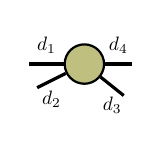
\begin{tikzpicture}[baseline=-0.5ex]
    \tikzset{tensor/.style = {minimum size = 0.5cm,shape = circle,thick,draw=black,inner sep = 0pt}, edge/.style = {thick,line width=.4mm},every loop/.style={}}
    \def\x{6}
    \def\y{0}
     \node[tensor,fill=green!50!red!50!white] (B) at (\x+1,\y) {$\Tt$};
    \draw[edge] (B) -- (\x+0.3,0) node [midway,above] {\scalebox{0.7}{\dimcolor{$d_1$}}};
    \draw[edge] (B) -- (\x+1.6,0) node [midway,above] {\scalebox{0.7}{\dimcolor{$d_4$}}};
    \draw[edge] (B) -- (\x+0.4,-0.3) node [midway, below] {\scalebox{0.7}{\dimcolor{$d_2$}}};
    \draw[edge] (B) -- (\x+1.5,-0.4)node [midway, below] {\scalebox{0.7}{\dimcolor{$d_3$}}};
\end{tikzpicture}
=
\begin{tikzpicture}[baseline=\baseline]
    \tikzset{tensor/.style = {minimum size = 0.5cm,shape = circle,thick,draw=black,inner sep = 0pt}, edge/.style   = {thick,line width=.4mm},every loop/.style={}}
    \def\y{0}
    \def\x{0}
  \node[tensor,fill=red!30!white] (D) at (\x-1,\y){$\Gt_1$};
  \node[tensor,fill=red!50!white] (A) at (\x,\y){\scalebox{0.85}{$\Gt_2$}};
  \node[tensor,fill=blue!50!white] (B) at (\x+1,\y){$\Gt_3$};
   \node[tensor,fill=blue!20!white] (C) at (\x+2,\y){$\Gt_4$};
    \draw[edge](A) -- (\x,\y-0.7)node [midway,left] {\edgelabel{$d_2$}};
    \draw[edge](B) -- (\x+1,\y-0.7)node [midway,left] {\edgelabel{$d_3$}};
    \draw[edge](C) -- (\x+2,\y-0.7)node [midway,left] {\edgelabel{$d_4$}};
     \draw[edge](D) -- (\x-1,\y-0.7)node [midway,left] {\edgelabel{$d_1$}};
    \draw[edge](D) -- (A) node [midway,above] {\edgelabel{$R_1$}};
    \draw[edge](A) -- (B) node [midway,above] {\edgelabel{$R_2$}};
    \draw[edge](B) -- (C) node [midway,above] {\edgelabel{$R_3$}};
\end{tikzpicture}.
\end{center}

由于 $\Tt$ 表示一个概率分布，它的元素必须非负，且总和为一。
在机器学习场景中，我们要针对某个损失函数~（如对数似然）来优化核心张量，此时可以对核心张量 $\Gt_1,\cdots,\Gt_N$ 施加若干约束以保证这两条性质。 
要保证 $\Tt$ 的元素非负，一个简单的办法是约束核心张量的元素非负，或者对所有核心张量的元素逐分量地施加一个取值非负的“激活”函数。另一种做法源于量子物理：假设 $\Tt$ 的元素是概率的平方根，而非概率本身： $\Tt_{i_1,\cdots,i_N} = \sqrt{\PP(X_1=i_1,\cdots,X_N=i_N)}$。当 $\Tt$ 处于 TT 格式时，这对应于如下张量网络：
$$
\PP(X_1=i_1,\cdots,X_4=i_4) = (\Tt_{i_1,\cdots,i_4})^2 = 
\begin{tikzpicture}[baseline=\baseline]
    \tikzset{tensor/.style = {minimum size = 0.5cm,shape = circle,thick,draw=black,inner sep = 0pt}, edge/.style   = {thick,line width=.4mm},every loop/.style={}}
    \def\y{-0.35}
    \def\x{0}
  \node[tensor,fill=red!30!white] (D) at (\x-1,\y){$\Gt_1$};
  \node[tensor,fill=red!50!white] (A) at (\x,\y){\scalebox{0.85}{$\Gt_2$}};
  \node[tensor,fill=blue!50!white] (B) at (\x+1,\y){$\Gt_3$};
   \node[tensor,fill=blue!20!white] (C) at (\x+2,\y){$\Gt_4$};
   \node[tensor,fill=red!30!white] (G1) at (\x-1,\y+0.85){$\Gt_1$};
  \node[tensor,fill=red!50!white] (G2) at (\x,\y+0.85){\scalebox{0.85}{$\Gt_2$}};
  \node[tensor,fill=blue!50!white] (G3) at (\x+1,\y+0.85){$\Gt_3$};
   \node[tensor,fill=blue!20!white] (G4) at (\x+2,\y+0.85){$\Gt_4$};
    \draw[edge](G1) -- (\x-1,\y+1.65)node [very near end, above]{\scalebox{0.7} {\indcolor{$i_1$}}};
    \draw[edge](G2) -- (\x,\y+1.65)node [very near end, above]{\scalebox{0.7} {\indcolor{$i_2$}}};
    \draw[edge](G3) -- (\x+1,\y+1.65)node [very near end, above]{\scalebox{0.7}{\indcolor{$i_3$}}};
    \draw[edge](G4) -- (\x+2,\y+1.65)node [very near end, above]{\scalebox{0.7}{\indcolor{$i_4$}}};
    \draw[edge](G1) -- (G2)node [midway,above] {\edgelabel{$R_1$}};
    \draw[edge](G2) -- (G3)node [midway,above] {\edgelabel{$R_2$}};
    \draw[edge](G3) -- (G4)node [midway,above] {\edgelabel{$R_3$}};
    \draw[edge](A) -- (\x,\y-0.7)node [very near end, below] {\scalebox{0.7}{\indcolor{$i_2$}}};
    \draw[edge](B) -- (\x+1,\y-0.7)node [very near end, below]{\scalebox{0.7} {\indcolor{$i_3$}}};
    \draw[edge](C) -- (\x+2,\y-0.7)node [very near end, below] {\scalebox{0.7}{\indcolor{$i_4$}}};
     \draw[edge](D) -- (\x-1,\y-0.7)node [very near end, below] {\scalebox{0.7}{\indcolor{$i_1$}}};
    \draw[edge](D) -- (A) node [midway,above] {\edgelabel{$R_1$}};
    \draw[edge](A) -- (B) node [midway,above] {\edgelabel{$R_2$}};
    \draw[edge](B) -- (C) node [midway,above] {\edgelabel{$R_3$}};
\end{tikzpicture}
.
$$

利用复制张量，我们可以将其写为：
\begin{align}\label{eqn:parametrized-prob}
    \PP(X_1,\cdots,X_4) \simeq
    \begin{tikzpicture}[baseline=\baseline]
    \tikzset{tensor/.style = {minimum size = 0.5cm,shape = circle,thick,draw=black,inner sep = 0pt}, edge/.style   = {thick,line width=.4mm},every loop/.style={}}
    \def\y{-0.35}
    \def\x{0}
  \node[tensor,fill=red!30!white] (D) at (\x-1,\y-0.25){$\Gt_1$};
  \node[tensor,fill=red!50!white] (A) at (\x,\y-0.25){\scalebox{0.85}{$\Gt_2$}};
  \node[tensor,fill=blue!50!white] (B) at (\x+1,\y-0.25){$\Gt_3$};
   \node[tensor,fill=blue!20!white] (C) at (\x+2,\y-0.25){$\Gt_4$};
   \node[tensor,fill=red!30!white] (G1) at (\x-1,\y+1){$\Gt_1$};
  \node[tensor,fill=red!50!white] (G2) at (\x,\y+1){\scalebox{0.85}{$\Gt_2$}};
  \node[tensor,fill=blue!50!white] (G3) at (\x+1,\y+1){$\Gt_3$};
   \node[tensor,fill=blue!20!white] (G4) at (\x+2,\y+1){$\Gt_4$};
    \draw[edge](G1) -- (G2)node [midway,above] {\edgelabel{$R_1$}};
    \draw[edge](G2) -- (G3)node [midway,above] {\edgelabel{$R_2$}};
    \draw[edge](G3) -- (G4)node [midway,above] {\edgelabel{$R_3$}};
    \draw[edge](D) -- (A) node [midway,above] {\edgelabel{$R_1$}};
    \draw[edge](A) -- (B) node [midway,above] {\edgelabel{$R_2$}};
    \draw[edge](B) -- (C) node [midway,above] {\edgelabel{$R_3$}};
    \draw  node[fill = black,circle,inner sep=0pt,minimum size=4pt] (m_1) at (\x-1,\y+0.35) {};
    \draw  node[fill = black,circle,inner sep=0pt,minimum size=4pt] (m_2) at (\x,\y+0.35) {};
    \draw  node[fill = black,circle,inner sep=0pt,minimum size=4pt] (m_3) at (\x+1,\y+0.35) {};
    \draw  node[fill = black,circle,inner sep=0pt,minimum size=4pt] (m_4) at (\x+2,\y+0.35) {};
    \draw[edge](D)--(G1);
    \draw[edge](A)--(G2);
    \draw[edge](B)--(G3);    \draw[edge](C)--(G4);
    \draw[edge](m_1) -- (\x-1.35,\y+0.35);
    \draw[edge](m_4) -- (\x+2.35,\y+0.35);
    \draw[edge](m_2) -- (\x-0.35,\y+0.35);
    \draw[edge](m_3) -- (\x+1.35,\y+0.35);
\end{tikzpicture}
\end{align}

为保证概率之和为一，我们可以选择建模未归一化的平方根概率，因为正如后文所见，当概率张量处于 TT 格式时，归一化常数的计算非常容易。于是我们假设
$$\PP(X_1=i_1,\cdots,X_N=i_N) = \frac{(\Tt_{i_1,\cdots,i_N})^2}{\zeta},$$
其中 $\zeta = \sum_{i_1,\cdots,i_N}(\Tt_{i_1,\cdots,i_N})^2$ 为归一化常数。与第~\ref{sec:efficient-operations} 节介绍的 TT 格式高效运算类似，该归一化因子同样可以在 TT 格式下高效计算： 
$$\zeta= \sum_{i_1,\cdots,i_4}\Tt_{i_1,\cdots,i_4}^2
=
\begin{tikzpicture}[baseline=\baseline]
    \tikzset{tensor/.style = {minimum size = 0.5cm,shape = circle,thick,draw=black,inner sep = 0pt}, edge/.style   = {thick,line width=.4mm},every loop/.style={}}
    \def\y{-0.35}
    \def\x{0}
  \node[tensor,fill=red!30!white] (D) at (\x-1,\y-0.25){$\Gt_1$};
  \node[tensor,fill=red!50!white] (A) at (\x,\y-0.25){\scalebox{0.85}{$\Gt_2$}};
    \node[tensor,fill=blue!50!white] (B) at (\x+1,\y-0.25){$\Gt_3$};
    \node[tensor,fill=blue!20!white] (C) at (\x+2,\y-0.25){$\Gt_4$};
     \node[tensor,fill=red!30!white] (G1) at (\x-1,\y+1){$\Gt_1$};
    \node[tensor,fill=red!50!white] (G2) at (\x,\y+1){\scalebox{0.85}{$\Gt_2$}};
    \node[tensor,fill=blue!50!white] (G3) at (\x+1,\y+1){$\Gt_3$};
    \node[tensor,fill=blue!20!white] (G4) at (\x+2,\y+1){$\Gt_4$};

    \draw[edge](G1) -- (G2)node [midway,above] {\edgelabel{$R_1$}};
    \draw[edge](G2) -- (G3)node [midway,above] {\edgelabel{$R_2$}};
    \draw[edge](G3) -- (G4)node [midway,above] {\edgelabel{$R_3$}};
    \draw[edge](D) -- (A) node [midway,above] {\edgelabel{$R_1$}};
    \draw[edge](A) -- (B) node [midway,above] {\edgelabel{$R_2$}};
    \draw[edge](B) -- (C) node [midway,above] {\edgelabel{$R_3$}};
    \draw[edge](G1)--(D);
    \draw[edge](G2)--(A);
    \draw[edge](G3)--(B);
    \draw[edge](G4)--(C);
\end{tikzpicture}.
$$
上述思想也被称为\emph{Born 机器}~\citep{glasser2019expressive,han2018unsupervised}。
与第~\ref{sub:probs} 节所示类似，TT 参数化的概率分布的边缘分布同样可以用张量网络来计算~（见式~\eqref{eqn:parametrized-prob}）：
\begin{enumerate}
    \item %
    利用全概率公式，$X_2,X_3$ 和 $X_4$ 的边缘分布可以表示为 
    \begin{align*}
    \PP(X_2=i_2, X_3=i_3, X_4=i_4) 
    &= \sum_{i_1=1}^{d_1}\PP(X_1=i_1,\cdots,X_4=i_4)\\ 
    &=
    \begin{tikzpicture}[baseline=\baseline]
    \tikzset{tensor/.style = {minimum size = 0.5cm,shape = circle,thick,draw=black,inner sep = 0pt}, edge/.style   = {thick,line width=.4mm},every loop/.style={}}
    \def\y{-0.35}
    \def\x{0}
  \node[tensor,fill=red!30!white] (D) at (\x-1,\y-0.25){$\Gt_1$};
  \node[tensor,fill=red!50!white] (A) at (\x,\y-0.25){\scalebox{0.85}{$\Gt_2$}};
  \node[tensor,fill=blue!50!white] (B) at (\x+1,\y-0.25){$\Gt_3$};
   \node[tensor,fill=blue!20!white] (C) at (\x+2,\y-0.25){$\Gt_4$};
   \node[tensor,fill=red!30!white] (G1) at (\x-1,\y+1){$\Gt_1$};
  \node[tensor,fill=red!50!white] (G2) at (\x,\y+1){\scalebox{0.85}{$\Gt_2$}};
  \node[tensor,fill=blue!50!white] (G3) at (\x+1,\y+1){$\Gt_3$};
   \node[tensor,fill=blue!20!white] (G4) at (\x+2,\y+1){$\Gt_4$};
    \draw[edge](G1) -- (G2)node [midway,above] {\edgelabel{$R_1$}};
    \draw[edge](G2) -- (G3)node [midway,above] {\edgelabel{$R_2$}};
    \draw[edge](G3) -- (G4)node [midway,above] {\edgelabel{$R_3$}};
    \draw[edge](D) -- (A) node [midway,above] {\edgelabel{$R_1$}};
    \draw[edge](A) -- (B) node [midway,above] {\edgelabel{$R_2$}};
    \draw[edge](B) -- (C) node [midway,above] {\edgelabel{$R_3$}};
    \draw  node[fill = black,circle,inner sep=0pt,minimum size=4pt] (m_1) at (\x-1,\y+0.35) {};
    \draw  node[fill = black,circle,inner sep=0pt,minimum size=4pt] (m_2) at (\x,\y+0.35) {};
    \draw  node[fill = black,circle,inner sep=0pt,minimum size=4pt] (m_3) at (\x+1,\y+0.35) {};
    \draw  node[fill = black,circle,inner sep=0pt,minimum size=4pt] (m_4) at (\x+2,\y+0.35) {};
    \draw[edge](D)--(G1);
    \draw[edge](A)--(G2);
    \draw[edge](B)--(G3);    \draw[edge](C)--(G4);
    \draw[edge](m_1) -- (\x-1.35,\y+0.35);
    \draw  node[fill = black,circle,inner sep=0pt,minimum size=4pt] (m) at (\x-1.35,\y+0.35) {};
    \draw[edge](m_4) -- (\x+2.35,\y+0.35) node [right] {\scalebox{0.7}{\indcolor{$i_4$}}};;
    \draw[edge](m_2) -- (\x-0.35,\y+0.35) node [left] {\scalebox{0.7}{\indcolor{$i_2$}}};;
    \draw[edge](m_3) -- (\x+1.35,\y+0.35) node [right] {\scalebox{0.7}{\indcolor{$i_3$}}};;
\end{tikzpicture}
=
\sum_{i_1}^{d_1}\Tt_{i_1,\cdots,i_4},
    \end{align*}
对任意 $i_2\in[d_1],i_3\in[d_3]$ 和 $i_4\in[d_4]$ 成立。 
\item 其余的边缘分布可以类似地表示。例如，$X_2$ 的边缘分布可以写为
\begin{align*}
    \PP(X_2=i_2) 
    &= \sum_{i_1,i_3,i_4=1}^{d_1,d_3,d_4}\PP(X_1=i_1,\cdots,X_4=i_4)\\ 
    &=
    \begin{tikzpicture}[baseline=\baseline]
    \tikzset{tensor/.style = {minimum size = 0.5cm,shape = circle,thick,draw=black,inner sep = 0pt}, edge/.style   = {thick,line width=.4mm},every loop/.style={}}
    \def\y{-0.35}
    \def\x{0}
  \node[tensor,fill=red!30!white] (D) at (\x-1,\y-0.25){$\Gt_1$};
  \node[tensor,fill=red!50!white] (A) at (\x,\y-0.25){\scalebox{0.85}{$\Gt_2$}};
  \node[tensor,fill=blue!50!white] (B) at (\x+1,\y-0.25){$\Gt_3$};
   \node[tensor,fill=blue!20!white] (C) at (\x+2,\y-0.25){$\Gt_4$};
   \node[tensor,fill=red!30!white] (G1) at (\x-1,\y+1){$\Gt_1$};
  \node[tensor,fill=red!50!white] (G2) at (\x,\y+1){\scalebox{0.85}{$\Gt_2$}};
  \node[tensor,fill=blue!50!white] (G3) at (\x+1,\y+1){$\Gt_3$};
   \node[tensor,fill=blue!20!white] (G4) at (\x+2,\y+1){$\Gt_4$};
    \draw[edge](G1) -- (G2)node [midway,above] {\edgelabel{$R_1$}};
    \draw[edge](G2) -- (G3)node [midway,above] {\edgelabel{$R_2$}};
    \draw[edge](G3) -- (G4)node [midway,above] {\edgelabel{$R_3$}};
    \draw[edge](D) -- (A) node [midway,above] {\edgelabel{$R_1$}};
    \draw[edge](A) -- (B) node [midway,above] {\edgelabel{$R_2$}};
    \draw[edge](B) -- (C) node [midway,above] {\edgelabel{$R_3$}};
    \draw  node[fill = black,circle,inner sep=0pt,minimum size=4pt] (m_1) at (\x-1,\y+0.35) {};
    \draw  node[fill = black,circle,inner sep=0pt,minimum size=4pt] (m_2) at (\x,\y+0.35) {};
    \draw  node[fill = black,circle,inner sep=0pt,minimum size=4pt] (m_3) at (\x+1,\y+0.35) {};
    \draw  node[fill = black,circle,inner sep=0pt,minimum size=4pt] (m_4) at (\x+2,\y+0.35) {};
    \draw[edge](D)--(G1);
    \draw[edge](A)--(G2);
    \draw[edge](B)--(G3);    
    \draw[edge](C)--(G4);
    \draw[edge](m_1) -- (\x-1.35,\y+0.35);
    \draw  node[fill = black,circle,inner sep=0pt,minimum size=4pt] (m_5) at (\x-1.35,\y+0.35) {};
    \draw[edge](m_4) -- (\x+2.35,\y+0.35);
    \draw  node[fill = black,circle,inner sep=0pt,minimum size=4pt] (m_6) at (\x+2.35,\y+0.35) {};
    \draw[edge](m_2) -- (\x-0.35,\y+0.35) node [left] {\scalebox{0.7}{\indcolor{$i_2$}}};;
    \draw[edge](m_3) -- (\x+1.35,\y+0.35);
    \draw  node[fill = black,circle,inner sep=0pt,minimum size=4pt] (m_7) at (\x+1.35,\y+0.35) {};
\end{tikzpicture}
=
\sum_{i_1,i_3,i_4=1}^{d_1,d_3,d_4}\Tt_{i_1,\cdots,i_4},
    \end{align*}
\end{enumerate}
\subsection{计算随机张量网络的期望} 
下面说明张量网络形式体系如何帮助我们推导随机张量的复杂性质。 
本节先给出两个非常有用的命题。
第一条只是期望的线性性的直接推论，但在本节中十分有用。
\begin{proposition}\label{prop:inner-expectation}
    设 $\At$ 与 $\Bt$ 为两个独立的随机张量网络。张量网络。则二者内积的期望为 
$$\EE\left(\begin{tikzpicture}[baseline=\baseline]
    \tikzset{tensor/.style = {minimum size = 0.5cm,shape = circle,thick,draw=black,inner sep = 0pt}, edge/.style = {thick,line width=.4mm},every loop/.style={}}
    \def\y{0}
    \def\x{0}
    \node[tensor,fill=red!50!blue!50!white] (At) at (\x,\y){\scalebox{0.85}{$\At$}};
    \node[tensor,fill=red!30!blue!50!white] (Bt) at (\x+1,\y){\scalebox{0.85}{$\Bt$}};
    \draw[edge] (At) -- (Bt);
    \draw[edge] (At) to [out=45,in=135] (Bt);
    \draw[edge] (At) to [out=-45,in=-135] (Bt);
    \draw[edge](At)--(\x-0.85,\y);
    \draw[edge](At)--(\x-0.75,\y+0.5);    \draw[edge](At)--(\x-0.75,\y-0.5);
    \draw[edge](Bt)--(\x+1.85,\y);
    \draw[edge](Bt)--(\x+1.75,\y+0.5);    \draw[edge](Bt)--(\x+1.75,\y-0.5);
\end{tikzpicture} \right)
=
\begin{tikzpicture}[baseline=\baseline]
    \tikzset{tensor/.style = {minimum size = 0.8cm,shape = circle,thick,draw=black,inner sep = 0pt}, edge/.style = {thick,line width=.4mm},every loop/.style={}}
    \def\y{0}
    \def\x{0}
    \node[tensor,fill=red!50!blue!50!white] (At) at (\x,\y){\scalebox{0.85}{$\EE(\At)$}};
    \node[tensor,fill=red!30!blue!50!white] (Bt) at (\x+1.5,\y){\scalebox{0.85}{$\EE(\Bt)$}};
    \draw[edge] (At) -- (Bt);
    \draw[edge] (At) to [out=45,in=135] (Bt);
    \draw[edge] (At) to [out=-45,in=-135] (Bt);
    \draw[edge](At)--(\x-0.85,\y);
    \draw[edge](At)--(\x-0.75,\y+0.5);    \draw[edge](At)--(\x-0.75,\y-0.5);
    \draw[edge](Bt)--(\x+2.35,\y);
    \draw[edge](Bt)--(\x+2.25,\y+0.5);    \draw[edge](Bt)--(\x+2.25,\y-0.5);
\end{tikzpicture}.
$$
\begin{proof}
结论直接由期望的线性性以及 $\At$ 与 $\Bt$ 的独立性得到。
\end{proof}
\end{proposition}
第二条给出一个有趣的性质：对于元素取自高斯分布的矩阵，其与自身的外积的期望归结为一个非常简单的张量网络。 
\begin{proposition}\label{prop:outer-prod}设 $\Ab\in\RR^{m\times n}$ 为随机矩阵，其元素独立同分布于标准正态分布。$\Ab$ 与自身的外积的期望为 
$$\EE\left(
\begin{tikzpicture}[baseline=\baseline]
    \tikzset{tensor/.style = {minimum size = 0.5cm,shape = circle,thick,draw=black,inner sep = 0pt}, edge/.style = {thick,line width=.4mm},every loop/.style={}}
    \def\y{0.15}
    \def\x{0}
    \node[tensor,fill=green!50!blue!20!white] (A) at (\x,\y){\scalebox{0.85}{$\Ab$}};
    \node[tensor,fill=green!50!blue!20!white] (B) at (\x+1.5,\y){\scalebox{0.85}{$\Ab$}};
    \draw[edge](A) -- (\x-0.55,\y-0.55);
    \node[draw=none] () at (\x-0.5,\y-0.3) {\scalebox{0.7}{\dimcolor{$m$}}};
    \draw[edge](A) -- (\x+0.55,\y-0.55);
    \node[draw=none] () at (\x+0.5,\y-0.3) {\scalebox{0.7}{\dimcolor{$n$}}};
    \draw[edge](B) -- (\x+1,\y-0.55);
    \node[draw=none] () at (\x+1,\y-0.3) {\scalebox{0.7}{\dimcolor{$m$}}};
    \draw[edge](B) -- (\x+2,\y-0.55);
    \node[draw=none] () at (\x+2,\y-0.3) {\scalebox{0.7}{\dimcolor{$n$}}};
\end{tikzpicture}
\right)
=
\begin{tikzpicture}[baseline=\baseline]
    \tikzset{tensor/.style = {minimum size = 0.5cm,shape = circle,thick,draw=black,inner sep = 0pt}, edge/.style = {thick,line width=.4mm},every loop/.style={}}
    \def\y{0}
    \def\x{0}
    \draw[edge] (\x+0.15,\y-0.1) to [out=100,in=80] (\x+1.85,\y-0.1);
    \draw[edge] (\x+1.45,\y-0.1) to [out=100,in=80] (\x+3,\y-0.1);
    \node[draw=none] () at (\x+2.25,\y+0.5) {\scalebox{0.6}{\dimcolor{$n$}}};
    \node[draw=none] () at (\x+1,\y+0.5) {\scalebox{0.6}{\dimcolor{$m$}}};
\end{tikzpicture},
$$
其中右端
是两个克罗内克 $\delta$ 的外积~（即 $
\begin{tikzpicture}[baseline=\baseline]
    \tikzset{tensor/.style = {minimum size = 0.5cm,shape = circle,thick,draw=black,inner sep = 0pt}, edge/.style = {thick,line width=.4mm},every loop/.style={}}
    \def\y{0}
    \def\x{0}
    \draw[edge] (\x+0.15,\y-0.1) to [out=100,in=80] (\x+1.85,\y-0.1);
    \draw[edge] (\x+1.45,\y-0.1) to [out=100,in=80] (\x+3,\y-0.1);
    \node[draw=none] () at (\x+0.15,\y-0.25) {\scalebox{0.7}{\indcolor{$i_1$}}};
    \node[draw=none] () at (\x+3,\y-0.25) {\scalebox{0.7}{\indcolor{$i_4$}}};
    \node[draw=none] () at (\x+1.85,\y-0.25) {\scalebox{0.7}{\indcolor{$i_3$}}};
    \node[draw=none] () at (\x+1.45,\y-0.25) {\scalebox{0.7}{\indcolor{$i_2$}}};
\end{tikzpicture}
=\delta_{i_1i_3}\delta_{i_2i_4}$，对任意 $i_1,i_3\in[m]$ 和 $i_2,i_4\in[n]$ 成立。）
\begin{proof}
由于 $\Ab$ 的元素独立取自 $\mathcal{N}(0,1)$，其向量化服从多元正态分布，$\vectorize(\Ab) \sim \mathcal{N}(\mathbf{0},\Ib_{mn})$，因而 $\EE(\vectorize(\Ab)\vectorize(\Ab)^\ts) = \Ib_{mn}$。这意味着 
$$ \EE(\Ab_{i_1i_2}\Ab_{i_3i_4})=
\begin{cases}
        1 & \text{ if } i_1=i_3\text{ and } i_2=i_4\\
        0 & \text{ otherwise, }
    \end{cases} 
    $$
于是 $\EE(\Ab\outprod\Ab)_{i_1i_2i_3i_4}=\EE(\Ab_{i_1i_2}\Ab_{i_3i_4}) = \delta_{i_1i_3}\delta_{i_2i_4}=
\begin{tikzpicture}[baseline=\baseline]
    \tikzset{tensor/.style = {minimum size = 0.5cm,shape = circle,thick,draw=black,inner sep = 0pt}, edge/.style = {thick,line width=.4mm},every loop/.style={}}
    \def\y{0}
    \def\x{0}
    \draw[edge] (\x+0.15,\y-0.1) to [out=100,in=80] (\x+1.85,\y-0.1);
    \draw[edge] (\x+1.45,\y-0.1) to [out=100,in=80] (\x+3,\y-0.1);
    \node[draw=none] () at (\x+0.15,\y-0.25) {\scalebox{0.7}{\indcolor{$i_1$}}};
    \node[draw=none] () at (\x+3,\y-0.25) {\scalebox{0.7}{\indcolor{$i_4$}}};
    \node[draw=none] () at (\x+1.85,\y-0.25) {\scalebox{0.7}{\indcolor{$i_3$}}};
    \node[draw=none] () at (\x+1.45,\y-0.25) {\scalebox{0.7}{\indcolor{$i_2$}}};
\end{tikzpicture}$，对任意 $i_1,i_3\in[m]$ 和 $i_2,i_4\in[n]$ 成立。


\end{proof}
\end{proposition}
\begin{remark}
    注意，$\EE(\Ab\outprod\Ab)$ 的指标不同排列顺序对应如下张量网络：  
    \begin{align*}
            \EE(\Ab\outprod\Ab)_{i_1i_2i_4i_3}
            &= 
            \EE(\Ab_{i_1i_2}\Ab_{i_4i_3}) 
    = \delta_{i_1i_4}\delta_{i_2i_3}\\
    &=
    \begin{cases}
        1 & \text{ if } i_1=i_4\text{ and } i_2=i_3\\
        0 & \text{ otherwise, }
    \end{cases} 
    =
    \begin{tikzpicture}[baseline=\baseline]
    \tikzset{tensor/.style = {minimum size = 0.5cm,shape = circle,thick,draw=black,inner sep = 0pt}, edge/.style = {thick,line width=.4mm},every loop/.style={}}
    \def\y{0}
    \def\x{0}
    \draw[edge] (\x,\y-0.1) to [out=100,in=80] (\x+2,\y-0.1);
    \draw[edge] (\x+0.15,\y-0.1) to [out=100,in=80] (\x+1.85,\y-0.1);
    \node[draw=none] () at (\x,\y-0.25) {\scalebox{0.7}{\indcolor{$i_1$}}};
    \node[draw=none] () at (\x+2.15,\y-0.25) {\scalebox{0.7}{\indcolor{$i_4$}}};
    \node[draw=none] () at (\x+0.35,\y-0.25) {\scalebox{0.7}{\indcolor{$i_2$}}};
    \node[draw=none] () at (\x+1.7,\y-0.25) {\scalebox{0.7}{\indcolor{$i_3$}}};
\end{tikzpicture},
    \end{align*}
以及
\begin{align*}
\EE(\Ab\outprod\Ab)_{i_1i_4i_2i_3} 
&= 
\EE(\Ab_{i_1i_4}\Ab_{i_2i_3})= \delta_{i_1i_2}\delta_{i_4i_3}\\
&=
\begin{cases}
        1 & \text{ if } i_1=i_2\text{ and } i_3=i_4\\
        0 & \text{ otherwise, }
\end{cases}
=
\begin{tikzpicture}[baseline=\baseline]
    \tikzset{tensor/.style = {minimum size = 0.5cm,shape = circle,thick,draw=black,inner sep = 0pt}, edge/.style = {thick,line width=.4mm},every loop/.style={}}
    \def\y{0}
    \def\x{0}
    \draw[edge] (\x+0.15,\y-0.1) to [out=100,in=80] (\x+1.85,\y-0.1);
    \draw[edge] (\x+2,\y-0.1) to [out=100,in=80] (\x+3.65,\y-0.1);
    \node[draw=none] () at (\x+0.15,\y-0.25) {\scalebox{0.7}{\indcolor{$i_1$}}};
    \node[draw=none] () at (\x+1.85,\y-0.25) {\scalebox{0.7}{\indcolor{$i_2$}}};
    \node[draw=none] () at (\x+2.15,\y-0.25) {\scalebox{0.7}{\indcolor{$i_3$}}};
    \node[draw=none] () at (\x+3.65,\y-0.25) {\scalebox{0.7}{\indcolor{$i_4$}}};
\end{tikzpicture}.
\end{align*}
\end{remark}
接下来说明如何借助命题~\ref{prop:inner-expectation} 与~\ref{prop:outer-prod}，为高斯随机矩阵与其自身乘积的期望给出一个极为简洁的张量网络推导。 
\begin{proposition}\label{prop:wishart-mean}
若随机矩阵 $\Ab\in\RR^{m\times n}$ 的元素独立同分布（i.i.d.）地取自标准正态分布，则 $\EE(\Ab^\ts\Ab) = m\Ib_n$。 
\begin{proof}
        借助命题~\ref{prop:inner-expectation} 与~\ref{prop:outer-prod}，可写为 
\begin{align*}
\EE(\Ab^\ts\Ab) 
&= 
\EE\left(\begin{tikzpicture}[baseline=\baseline]
    \tikzset{tensor/.style = {minimum size = 0.5cm,shape = circle,thick,draw=black,inner sep = 0pt}, edge/.style = {thick,line width=.4mm},every loop/.style={}}
    \def\y{0}
    \def\x{0}
    \node[tensor,fill=red!30!blue!30!white] (A1) at (\x,\y){\scalebox{0.85}{$\Ab$}};
    \node[tensor,fill=red!30!blue!30!white] (A2) at (\x+1,\y){\scalebox{0.85}{$\Ab$}};
    \draw[edge](A1) -- (A2) node [midway, above]{\scalebox{0.7}{\dimcolor{$m$}}};
    \draw[edge](A1) -- (\x-0.85,\y) node [midway, above]{\scalebox{0.7}{\dimcolor{$n$}}};
    \draw[edge](A2) -- (\x+1.85,\y) node [midway, above]{\scalebox{0.7}{\dimcolor{$n$}}};
\end{tikzpicture}\right)
=
\EE\left(\begin{tikzpicture}[baseline=\baseline]
    \tikzset{tensor/.style = {minimum size = 0.5cm,shape = circle,thick,draw=black,inner sep = 0pt}, edge/.style = {thick,line width=.4mm},every loop/.style={}}
    \def\y{0}
    \def\x{0}
    \node[tensor,fill=red!30!blue!30!white] (A2) at (\x,\y-0.5){\scalebox{0.85}{$\Ab$}};
    \node[tensor,fill=red!30!blue!30!white] (A1) at (\x,\y+0.5){\scalebox{0.85}{$\Ab$}};
    \draw[edge](\x+0.25,\y+0.4) -- (\x+1.25,\y+0.4) -- (\x+1.25,\y-0.4) -- (\x+0.25,\y-0.4);
    \draw[edge](\x+0.2,\y+0.65)--(\x+1.25,\y+0.65)node [midway, above]{\scalebox{0.7}{\dimcolor{$n$}}};
    \draw[edge](\x+0.2,\y-0.65)--(\x+1.25,\y-0.65)node [midway, below]{\scalebox{0.7}{\dimcolor{$n$}}};
    \node[draw=none] () at (\x+1.45,\y) {\scalebox{0.7}{\dimcolor{$m$}}};
    \draw[dotted](\x+0.55,\y+1)--(\x+0.55,\y-1);
\end{tikzpicture}\right)\\
\ \
&\textequal{Prop.~\ref{prop:inner-expectation}}
\ \
\begin{tikzpicture}[baseline=\baseline]
   \tikzset{tensor/.style = {minimum size = 0.5cm,shape = circle,thick,draw=black,inner sep = 0pt}, edge/.style = {thick,line width=.4mm},every loop/.style={}}
    \def\y{0}
    \def\x{0}
    \node[tensor,fill=red!30!blue!30!white] (A1) at (\x,\y+0.5){\scalebox{0.85}{$\Ab$}};
    \node[tensor,fill=red!30!blue!30!white] (A2) at (\x,\y-0.5){\scalebox{0.85}{$\Ab$}};
    \draw[edge,draw=blue](\x+0.25,\y+0.4) -- (\x+1.65,\y+0.4);
    \draw[edge, draw=red](\x+1.65,\y+0.4)-- (\x+1.95,\y+0.4) -- (\x+1.95,\y-0.4)--(\x+1.65,\y+0-0.4);
    \draw[edge, draw=blue](\x+1.65,\y-0.4) -- (\x+0.25,\y-0.4);
    \draw[edge, draw=blue](\x+0.2,\y+0.65)--(\x+1.95,\y+0.65)node [midway, above]{\scalebox{0.7}{\dimcolor{$n$}}};
    \draw[edge,draw=blue](\x+0.2,\y-0.65)--(\x+1.95,\y-0.65)node [midway, below]{\scalebox{0.7}{\dimcolor{$n$}}};
    \node[draw=none] () at (\x+2.15,\y) {\scalebox{0.7}{\dimcolor{$m$}}};
    \node at (\x-0.55,\y) {$\EE\left( \vphantom{\rule{0pt}{1cm}} \right.$};
    \node at (\x+0.55,\y) {$\left. \vphantom{\rule{0pt}{1cm}} \right)$};
    \node at (\x+1.15,\y) {$\EE\left( \vphantom{\rule{0pt}{1cm}} \right.$};
    \node at (\x+2.35,\y) {$\left. \vphantom{\rule{0pt}{1cm}} \right)$};
\end{tikzpicture}
~~\textequal{Prop.~\ref{prop:outer-prod}}
\ \ 
\begin{tikzpicture}[baseline=\baseline]
   \tikzset{tensor/.style = {minimum size = 0.5cm,shape = circle,thick,draw=black,inner sep = 0pt}, edge/.style = {thick,line width=.4mm},every loop/.style={}}
    \def\y{0}
    \def\x{0}
    \draw[edge,draw=blue](\x+1.35,\y+0.4) -- (\x+1.65,\y+0.4);
    \draw[edge, draw=red](\x+1.65,\y+0.4)-- (\x+1.95,\y+0.4) -- (\x+1.95,\y-0.4)--(\x+1.65,\y+0-0.4);
    \draw[edge, draw=blue](\x+1.35,\y-0.4) -- (\x+1.65,\y-0.4);
    \draw[edge, draw=blue](\x+1.35,\y-0.4) -- (\x+1.35,\y-0.4);
    \draw[edge, draw=blue](\x+1.35,\y+0.65)--(\x+1.95,\y+0.65);
    \draw[edge,draw=blue](\x+1.35,\y-0.65)--(\x+1.95,\y-0.65);
    \node[draw=none] () at (\x+2.15,\y) {\scalebox{0.7}{\dimcolor{$m$}}};
    \node[draw=none] () at (\x+1.35,\y) {\scalebox{0.7}{\dimcolor{$m$}}};
    \node[draw=none] () at (\x+0.85,\y) {\scalebox{0.7}{\dimcolor{$n$}}};
    \draw[edge, draw=blue](\x+1.35,\y+0.65)to[out=170,in=190](\x+1.35,\y-0.65);
    \draw[edge, draw=blue](\x+1.35,\y+0.4)to[out=190,in=170](\x+1.35,\y-0.4);
\end{tikzpicture}
= m\Ib_n.
\end{align*}
最后一个图由收缩长度为 $m$ 的腿得到。可以看到，一旦完成收缩，所得表达式就是单位矩阵的迹，对应上面等式中长度为 $m$ 的圆环。
\end{proof}
\end{proposition}
上述命题可解释为关于 Wishart 分布均值的陈述。  
回顾一下，从 Wishart 分布 $W_p(\mat \Sigma, m)$（其中 $\mat \Sigma \in \RR^{n\times n}$ 为协方差矩阵）采样矩阵 $\mat X$ 的做法是：把矩阵 $\mat A\in\mathbb R^{m\times n}$ 的每一列独立地取自多元正态 $\mathcal N(\vec 0 , \mat \Sigma)$，再令 $\mat X = \mat A^\top\mat A$。因此，命题~\ref{prop:inner-expectation} 中的矩阵 $\Ab ^\top \Ab$ 服从 Wishart 分布  $W_p(\mat I,m)$。
\begin{remark} 由命题~\ref{prop:inner-expectation} 可知，若 $\Ab \in \RR^{m \times n}$ 的元素取自标准正态分布，则 $\EE(\norm{\Ab}_F^2) = mn$。 
该结论可推广到元素独立同分布地取自标准正态分布的高阶张量，例如若 $\Tt\in\RR^{d_1\times d_2\times\cdots\times d_N}$，则 $\EE(\norm{\Tt}_F^2) = d_1d_2\cdots d_N$。
\end{remark}
利用前述命题给出的高斯随机矩阵性质，可以计算其乘积的期望范数。同样地，用张量网络表述后证明极为简洁，而若用指标与求和显式处理，则要繁琐得多。
\begin{proposition}\label{prop:expected-norm}
    设 $\Ab\in\RR^{m\times r}$ 与 $\Bb\in\RR^{r\times n}$ 为随机矩阵，其元素独立同分布（i.i.d.）于均值为零、方差为一的标准正态分布。则其乘积的 Frobenius 范数平方的期望为 $\EE({\norm{\Ab\Bb}^2_F}) = mnr$。
\begin{proof}
借助命题~\ref{prop:inner-expectation}，可写为
\begin{align*}
 \EE({\norm{\Ab\Bb}^2_F})
 &= 
 \EE\left(\begin{tikzpicture}[baseline=\baseline]
   \tikzset{tensor/.style = {minimum size = 0.5cm,shape = circle,thick,draw=black,inner sep = 0pt}, edge/.style = {thick,line width=.4mm},every loop/.style={}}
    \def\y{0}
    \def\x{0}
    \node[tensor,fill=red!50!white] (A) at (\x,\y+0.5){\scalebox{0.85}{$\Ab$}};
    \node[tensor,fill=blue!50!white] (B) at (\x+1,\y+0.5){\scalebox{0.85}{$\Bb$}};
    \draw[edge] (A) -- (B) node [midway,above]{\scalebox{0.7}{\dimcolor{$r$}}};
    \node[tensor,fill=red!50!white] (A1) at (\x,\y-0.5){\scalebox{0.85}{$\Ab$}};
    \node[tensor,fill=blue!50!white] (B1) at (\x+1,\y-0.5){\scalebox{0.85}{$\Bb$}};
    \draw[edge] (A1) -- (B1) node [midway,above]{\scalebox{0.7}{\dimcolor{$r$}}};
    \draw[edge] (A) to [out=-150,in=160, distance=0.5cm] (A1);
    \draw[edge] (B) to [out=-30,in=20, distance=0.5cm] (B1);
    \node[draw=none] () at (\x-0.75,\y) {\scalebox{0.7}{\dimcolor{$m$}}};
    \node[draw=none] () at (\x+1.75,\y) {\scalebox{0.7}{\dimcolor{$n$}}};
    \end{tikzpicture}\right)\\
&=
\EE\left(\begin{tikzpicture}[baseline=\baseline]
   \tikzset{tensor/.style = {minimum size = 0.5cm,shape = circle,thick,draw=black,inner sep = 0pt}, edge/.style = {thick,line width=.4mm},every loop/.style={}}
    \def\y{0.25}
    \def\x{0}
    \node[tensor,fill=red!50!white] (A) at (\x,\y){\scalebox{0.85}{$\Ab$}}; 
    \node[tensor,fill=red!50!white] (A1) at (\x+1,\y){\scalebox{0.85}{$\Ab$}};
    \draw[edge](A)--(A1)node[midway,above] {\scalebox{0.7}{\dimcolor{$m$}}};
    \draw[edge](A)--(\x,\y-0.85)node[midway,left] {\scalebox{0.7}{\dimcolor{$r$}}};
    \draw[edge](A1)--(\x+1,\y-0.85)node[midway,right] {\scalebox{0.7}{\dimcolor{$r$}}};
    \node[tensor,fill=blue!50!white] (B) at (\x+2,\y){\scalebox{0.85}{$\Bb$}}; 
    \node[tensor,fill=blue!50!white] (B1) at (\x+3,\y){\scalebox{0.85}{$\Bb$}};
    \draw[edge](B)--(B1)node[midway,above] {\scalebox{0.7}{\dimcolor{$n$}}};
    \draw[edge](B)--(\x+2,\y-0.85)node[midway,left] {\scalebox{0.7}{\dimcolor{$r$}}};
    \draw[edge](B1)--(\x+3,\y-0.85)node[midway,right] {\scalebox{0.7}{\dimcolor{$r$}}};
    \draw[edge](\x+2,\y-0.85) -- (\x+2,\y-1) -- (\x+1,\y-1) -- (\x+1,\y-0.85);
    \draw[edge](\x+3,\y-0.85) -- (\x+3,\y-1.25) -- (\x,\y-1.25) -- (\x,\y-0.85);
    \draw[dotted](\x+1.5,\y+0.5) -- (\x+1.5,\y-1.65);
\end{tikzpicture}\right)
=
\begin{tikzpicture}[baseline=\baseline]
   \tikzset{tensor/.style = {minimum size = 0.5cm,shape = circle,thick,draw=black,inner sep = 0pt}, edge/.style = {thick,line width=.4mm},every loop/.style={}}
    \def\y{0}
    \def\x{0}
    \node[tensor,fill=red!50!white] (A) at (\x,\y){\scalebox{0.85}{$\Ab$}}; 
    \node[tensor,fill=red!50!white] (A1) at (\x+1,\y){\scalebox{0.85}{$\Ab$}};
    \draw[edge, draw=red](A)--(A1)node[midway,above] {\scalebox{0.7}{\dimcolor{$m$}}};
   \node[tensor,fill=blue!50!white] (B) at (\x+2,\y){\scalebox{0.85}{$\Bb$}}; 
    \node[tensor,fill=blue!50!white] (B1) at (\x+3,\y){\scalebox{0.85}{$\Bb$}};
    \draw[edge, draw=blue](B)--(B1)node[midway,above] {\scalebox{0.7}{\dimcolor{$n$}}};
    \node at (\x-0.55,\y) {$\EE\Biggl ( $};
    \node (eq) at (\x+1.39,\y) {$\Biggr )\EE$};
    \node (eq) at (\x+1.73,\y) {$\Biggl($};
    \draw[edge, draw=blue](B) -- (\x+2,\y-0.85);
    \draw[edge, draw=blue](B1) -- (\x+3,\y-0.85);
    \draw[edge, draw=red](A) -- (\x,\y-0.85);
    \draw[edge, draw=red](A1) -- (\x+1,\y-0.85);
    \draw[edge](\x+1,\y-0.85) -- (\x+1,\y-1) -- (\x+2,\y-1)--(\x+2,\y-0.85);
    \draw[edge](\x+3,\y-0.85) -- (\x+3,\y-1.2) -- (\x,\y-1.2) -- (\x,\y-0.85);
    \node[draw=none] () at (\x+1.65,\y-0.85) {\scalebox{0.7}{\dimcolor{$r$}}};
    \node[draw=none] () at (\x+0.5,\y-0.95) {\scalebox{0.7}{\dimcolor{$r$}}};
\end{tikzpicture}\Biggr).
\end{align*}
由命题~\ref{prop:wishart-mean} 有 $\EE\left(\begin{tikzpicture}[baseline=\baseline]
   \tikzset{tensor/.style = {minimum size = 0.5cm,shape = circle,thick,draw=black,inner sep = 0pt}, edge/.style = {thick,line width=.4mm},every loop/.style={}}
    \def\y{0.15}
    \def\x{0}
    \node[tensor,fill=red!50!white] (A) at (\x,\y){\scalebox{0.85}{$\Ab$}}; 
    \node[tensor,fill=red!50!white] (A1) at (\x+1,\y){\scalebox{0.85}{$\Ab$}};
    \draw[edge, draw=red](A)--(A1)node[midway,above] {\scalebox{0.7}{\dimcolor{$m$}}};
    \draw[edge, draw=red](A) -- (\x,\y-0.85)node[midway,left] {\scalebox{0.7}{\dimcolor{$r$}}};
    \draw[edge, draw=red](A1) -- (\x+1,\y-0.85)node[midway,right] {\scalebox{0.7}{\dimcolor{$r$}}};
\end{tikzpicture}\right)
=
m\begin{tikzpicture}[baseline=\baseline]
   \tikzset{tensor/.style = {minimum size = 0.5cm,shape = circle,thick,draw=black,inner sep = 0pt}, edge/.style = {thick,line width=.4mm},every loop/.style={}}
    \def\y{0}
    \def\x{0}
     \draw[edge, draw=red] (\x,\y-0.1) to [out=100,in=80] (\x+2,\y-0.1);
    \node[draw=none] () at (\x+1,\y+0.65) {\scalebox{0.7}{\dimcolor{$r$}}};
\end{tikzpicture}$
以及 
$\EE\left(\begin{tikzpicture}[baseline=\baseline]
   \tikzset{tensor/.style = {minimum size = 0.5cm,shape = circle,thick,draw=black,inner sep = 0pt}, edge/.style = {thick,line width=.4mm},every loop/.style={}}
    \def\y{0.15}
    \def\x{0}
    \node[tensor,fill=blue!50!white] (B) at (\x,\y){\scalebox{0.85}{$\Bb$}}; 
    \node[tensor,fill=blue!50!white] (B1) at (\x+1,\y){\scalebox{0.85}{$\Bb$}};
    \draw[edge, draw=blue](B)--(B1)node[midway,above] {\scalebox{0.7}{\dimcolor{$n$}}};
    \draw[edge, draw=blue](B) -- (\x,\y-0.85)node[midway,left] {\scalebox{0.7}{\dimcolor{$r$}}};
    \draw[edge, draw=blue](B1) -- (\x+1,\y-0.85)node[midway,right] {\scalebox{0.7}{\dimcolor{$r$}}};
\end{tikzpicture}\right)
= 
n\begin{tikzpicture}[baseline=\baseline]
   \tikzset{tensor/.style = {minimum size = 0.5cm,shape = circle,thick,draw=black,inner sep = 0pt}, edge/.style = {thick,line width=.4mm},every loop/.style={}}
    \def\y{0}
    \def\x{0}
     \draw[edge, draw=blue] (\x,\y-0.1) to [out=100,in=80] (\x+2,\y-0.1);
    \node[draw=none] () at (\x+1,\y+0.65) {\scalebox{0.7}{\dimcolor{$r$}}};
\end{tikzpicture}.
$ 
由于长度为 $r$ 的腿之间存在收缩，最终得到
\begin{align*}
 \EE({\norm{\Ab\Bb}^2_F})
 = 
 \EE\left(\begin{tikzpicture}[baseline=\baseline]
   \tikzset{tensor/.style = {minimum size = 0.5cm,shape = circle,thick,draw=black,inner sep = 0pt}, edge/.style = {thick,line width=.4mm},every loop/.style={}}
    \def\y{0}
    \def\x{0}
    \node[tensor,fill=red!50!white] (A) at (\x,\y+0.5){\scalebox{0.85}{$\Ab$}};
    \node[tensor,fill=blue!50!white] (B) at (\x+1,\y+0.5){\scalebox{0.85}{$\Bb$}};
    \draw[edge] (A) -- (B) node [midway,above]{\scalebox{0.7}{\dimcolor{$r$}}};
    \node[tensor,fill=red!50!white] (A1) at (\x,\y-0.5){\scalebox{0.85}{$\Ab$}};
    \node[tensor,fill=blue!50!white] (B1) at (\x+1,\y-0.5){\scalebox{0.85}{$\Bb$}};
    \draw[edge] (A1) -- (B1) node [midway,above]{\scalebox{0.7}{\dimcolor{$r$}}};
    \draw[edge] (A) to [out=-150,in=160, distance=0.5cm] (A1);
    \draw[edge] (B) to [out=-30,in=20, distance=0.5cm] (B1);
    \node[draw=none] () at (\x-0.75,\y) {\scalebox{0.7}{\dimcolor{$m$}}};
    \node[draw=none] () at (\x+1.75,\y) {\scalebox{0.7}{\dimcolor{$n$}}};
    \end{tikzpicture}\right)
=
mn\  \begin{tikzpicture}     [baseline=\baseline]
 \tikzset{tensor/.style = {minimum size = 0.5cm,shape = circle,thick,draw=black,inner sep = 0pt}, edge/.style = {thick,line 
width=.4mm},every loop/.style={}}
    \def\y{0}
    \def\x{1}
    \draw[edge](\x+2,\y) -- (\x+2,\y-0.35) -- (\x+3,\y-0.35)--(\x+3,\y);
    \draw[edge](\x+1,\y) -- (\x+1,\y-0.5) -- (\x+4,\y-0.5) -- (\x+4,\y);
    \draw[edge, draw=red] (\x+2,\y) to [out=100,in=80](\x+1,\y);
    \draw[edge, draw=blue] (\x+3,\y) to [out=100,in=80](\x+4,\y);
    \node[draw=none] () at (\x+2.5,\y-0.65) {\scalebox{0.7}{\dimcolor{$r$}}};
    \node[draw=none] () at (\x+3.5,\y+0.5) {\scalebox{0.7}{\dimcolor{$r$}}};
    \node[draw=none] () at (\x+1.5,\y+0.5) {\scalebox{0.7}{\dimcolor{$r$}}};
\end{tikzpicture}
= mnr.
\end{align*}
\end{proof}
\end{proposition}
掌握了高斯随机矩阵乘积期望范数的计算方法后，便可把这一方法推广到更复杂的张量网络的期望。

\paragraph{例} 设有一个任意的张量网络，例如
$$\Tt = 
\begin{tikzpicture}[baseline=\baseline]
   \tikzset{tensor/.style = {minimum size = 0.5cm,shape = circle,thick,draw=black,inner sep = 0pt}, edge/.style = {thick,line width=.4mm},every loop/.style={}}
    \def\y{0}
    \def\x{0}
    \node[tensor,fill=red!20!blue!20!white] (A) at (\x,\y){\scalebox{0.85}{$\At$}}; 
    \node[tensor,fill=red!40!blue!20!white] (B) at (\x+1,\y){\scalebox{0.85}{$\Bt$}};
    \node[tensor,fill=red!40!blue!30!white] (C) at (\x+2,\y){\scalebox{0.85}{$\Ct$}};
    \node[tensor,fill=red!60!blue!40!white] (G) at (\x+1,\y+1){\scalebox{0.85}{$\Gt$}};
    \draw[edge](A)--(B)node[midway,above] {\scalebox{0.7}{\dimcolor{$r_1$}}};
    \draw[edge](B)--(C)node[midway,above] {\scalebox{0.7}{\dimcolor{$r_2$}}};
    \draw[edge](G)--(A)node[midway,left] {\scalebox{0.7}{\dimcolor{$d_1$}}};
    \draw[edge](G)--(B)node[midway,left] {\scalebox{0.7}{\dimcolor{$d_2$}}};
    \draw[edge](G)--(C)node[midway,right] {\scalebox{0.7}{\dimcolor{$d_3$}}};
    \draw[edge](A)--(\x,\y-0.85)node[midway,left] {\scalebox{0.7}{\dimcolor{$m_1$}}};
    \draw[edge](B)--(\x+1,\y-0.85)node[midway,left] {\scalebox{0.7}{\dimcolor{$m_2$}}};
    \draw[edge](C)--(\x+2,\y-0.85)node[midway,left] {\scalebox{0.7}{\dimcolor{$m_3$}}};
\end{tikzpicture},
$$
其中 $\At\in\RR^{m_1\times d_1\times r_1}, \Bt\in\RR^{m_2\times r_1\times d_2\times r_2}, \Ct\in\RR^{m_3\times r_2\times d_3}$ 与 $\Gt\in\RR^{d_1\times d_2\times d_3}$ 的元素均独立同分布地取自标准正态分布，我们要计算 $\norm{\Tt}^2_F$ 的期望。利用张量网络图，有
\begin{align*}
    \EE\left(\norm{\begin{tikzpicture}[baseline=\baseline]
   \tikzset{tensor/.style = {minimum size = 0.5cm,shape = circle,thick,draw=black,inner sep = 0pt}, edge/.style = {thick,line width=.4mm},every loop/.style={}}
    \def\y{0}
    \def\x{0}
    \node[tensor,fill=red!20!blue!20!white] (A) at (\x,\y){\scalebox{0.85}{$\At$}}; 
    \node[tensor,fill=red!40!blue!20!white] (B) at (\x+1,\y){\scalebox{0.85}{$\Bt$}};
    \node[tensor,fill=red!40!blue!30!white] (C) at (\x+2,\y){\scalebox{0.85}{$\Ct$}};
    \node[tensor,fill=red!60!blue!40!white] (G) at (\x+1,\y+1){\scalebox{0.85}{$\Gt$}};
    \draw[edge](A)--(B)node[midway,above] {\scalebox{0.7}{\dimcolor{$r_1$}}};
    \draw[edge](B)--(C)node[midway,above] {\scalebox{0.7}{\dimcolor{$r_2$}}};
    \draw[edge](G)--(A)node[midway,left] {\scalebox{0.7}{\dimcolor{$d_1$}}};
    \draw[edge](G)--(B)node[midway,left] {\scalebox{0.7}{\dimcolor{$d_2$}}};
    \draw[edge](G)--(C)node[midway,right] {\scalebox{0.7}{\dimcolor{$d_3$}}};
    \draw[edge](A)--(\x,\y-0.85)node[midway,left] {\scalebox{0.7}{\dimcolor{$m_1$}}};
    \draw[edge](B)--(\x+1,\y-0.85)node[midway,left] {\scalebox{0.7}{\dimcolor{$m_2$}}};
    \draw[edge](C)--(\x+2,\y-0.85)node[midway,left] {\scalebox{0.7}{\dimcolor{$m_3$}}};
\end{tikzpicture}}_F^2\right)
=
\EE\left(\begin{tikzpicture}[baseline=\baseline]
   \tikzset{tensor/.style = {minimum size = 0.5cm,shape = circle,thick,draw=black,inner sep = 0pt}, edge/.style = {thick,line width=.4mm},every loop/.style={}}
    \def\y{0.5}
    \def\x{0}
    \node[tensor,fill=red!20!blue!20!white] (A_1) at (\x,\y){\scalebox{0.85}{$\At$}}; 
    \node[tensor,fill=red!40!blue!20!white] (B_1) at (\x+1,\y){\scalebox{0.85}{$\Bt$}};
    \node[tensor,fill=red!40!blue!30!white] (C_1) at (\x+2,\y){\scalebox{0.85}{$\Ct$}};
    \node[tensor,fill=red!60!blue!40!white] (G_1) at (\x+1,\y+1){\scalebox{0.85}{$\Gt$}};
    \draw[edge](A_1)--(B_1)node[midway,above] {\scalebox{0.7}{\dimcolor{$r_1$}}};
    \draw[edge](B_1)--(C_1)node[midway,above] {\scalebox{0.7}{\dimcolor{$r_2$}}};
    \draw[edge](G_1)--(A_1)node[midway,left] {\scalebox{0.7}{\dimcolor{$d_1$}}};
    \draw[edge](G_1)--(B_1)node[midway,left] {\scalebox{0.7}{\dimcolor{$d_2$}}};
    \draw[edge](G_1)--(C_1)node[midway,right] {\scalebox{0.7}{\dimcolor{$d_3$}}};
    \node[tensor,fill=red!20!blue!20!white] (A) at (\x,\y-1){\scalebox{0.85}{$\At$}}; 
    \node[tensor,fill=red!40!blue!20!white] (B) at (\x+1,\y-1){\scalebox{0.85}{$\Bt$}};
    \node[tensor,fill=red!40!blue!30!white] (C) at (\x+2,\y-1){\scalebox{0.85}{$\Ct$}};
    \node[tensor,fill=red!60!blue!40!white] (G) at (\x+1,\y-2){\scalebox{0.85}{$\Gt$}};
    \draw[edge](A)--(B)node[midway,above] {\scalebox{0.7}{\dimcolor{$r_1$}}};
    \draw[edge](B)--(C)node[midway,above] {\scalebox{0.7}{\dimcolor{$r_2$}}};
    \draw[edge](G)--(A)node[midway,left] {\scalebox{0.7}{\dimcolor{$d_1$}}};
    \draw[edge](G)--(B)node[midway,left] {\scalebox{0.7}{\dimcolor{$d_2$}}};
    \draw[edge](G)--(C)node[midway,right] {\scalebox{0.7}{\dimcolor{$d_3$}}};
    \draw[edge](A_1)--(A)node[midway,left] {\scalebox{0.7}{\dimcolor{$m_1$}}};
    \draw[edge](B_1)--(B)node[midway,left] {\scalebox{0.7}{\dimcolor{$m_2$}}};
    \draw[edge](C_1)--(C)node[midway,left] {\scalebox{0.7}{\dimcolor{$m_3$}}};
\end{tikzpicture}\right).
\end{align*}
由命题~\ref{prop:wishart-mean} 可知 

$$
\EE\left(\begin{tikzpicture}[baseline=\baseline]
   \tikzset{tensor/.style = {minimum size = 0.5cm,shape = circle,thick,draw=black,inner sep = 0pt}, edge/.style = {thick,line width=.4mm},every loop/.style={}}
    \def\y{0.5}
    \def\x{0}
    \node[tensor,fill=red!20!blue!20!white] (A1) at (\x,\y){\scalebox{0.85}{$\At$}}; 
    \node[tensor,fill=red!20!blue!20!white] (A2) at (\x,\y-1){\scalebox{0.85}{$\At$}}; 
    \draw[edge, draw=blue](A1) -- (A2)node [midway,right]{\scalebox{0.7}{\dimcolor{$m_1$}}};
    \draw[edge, draw=blue](A1) -- (\x+0.65,\y)node [midway,above]{\scalebox{0.7}{\dimcolor{$r_1$}}};
    \draw[edge, draw=blue](A2) -- (\x+0.65,\y-1)node [midway,above]{\scalebox{0.7}{\dimcolor{$r_1$}}};
    \draw[edge,draw=blue](A1) -- (\x,\y+0.65)node [midway,right]{\scalebox{0.7}{\dimcolor{$d_1$}}};
    \draw[edge,draw=blue](A2) -- (\x,\y-1.65)node [midway,right]{\scalebox{0.7}{\dimcolor{$d_1$}}};
\end{tikzpicture}\right) = m_1
\begin{tikzpicture}[baseline=\baseline]
   \tikzset{tensor/.style = {minimum size = 0.5cm,shape = circle,thick,draw=black,inner sep = 0pt}, edge/.style = {thick,line width=.4mm},every loop/.style={}}
    \def\y{0}
    \def\x{0}
    \draw[edge, draw=blue](\x-0.65,\y+0.5) -- (\x-0.65,\y-0.5);
    \draw[edge, draw=blue](\x,\y+0.5) to [out=190,in=170] (\x,\y-0.5);
    \node[draw=none] () at (\x-0.8,\y) {\scalebox{0.7}{\dimcolor{$d_1$}}};
    \node[draw=none] () at (\x-0.1,\y) {\scalebox{0.7}{\dimcolor{$r_1$}}};
\end{tikzpicture},\  
\EE\left(\begin{tikzpicture}[baseline=\baseline]
   \tikzset{tensor/.style = {minimum size = 0.5cm,shape = circle,thick,draw=black,inner sep = 0pt}, edge/.style = {thick,line width=.4mm},every loop/.style={}}
    \def\y{0.5}
    \def\x{0}
    \node[tensor,fill=red!40!blue!20!white] (B1) at (\x,\y){\scalebox{0.85}{$\Bt$}};
    \node[tensor,fill=red!40!blue!20!white] (B2) at (\x,\y-1){\scalebox{0.85}{$\Bt$}};
    \draw[edge, draw=red](B1) -- (B2)node [midway,right]{\scalebox{0.7}{\dimcolor{$m_2$}}};
    \draw[edge, draw=red](B1) -- (\x,\y+0.65)node [midway,right]{\scalebox{0.7}{\dimcolor{$d_2$}}};
    \draw[edge, draw=red](B1) -- (\x+0.65,\y)node [midway,above]{\scalebox{0.7}{\dimcolor{$r_2$}}};
    \draw[edge, draw=red](B2) -- (\x+0.65,\y-1)node [midway,above]{\scalebox{0.7}{\dimcolor{$r_2$}}};
    \draw[edge, draw=red](B1) -- (\x-0.65,\y)node [midway,above]{\scalebox{0.7}{\dimcolor{$r_1$}}};
    \draw[edge, draw=red](B2) -- (\x-0.65,\y-1)node [midway,above]{\scalebox{0.7}{\dimcolor{$r_1$}}};
     \draw[edge, draw=red](B2) --(\x,\y-1.65)node [midway,right]{\scalebox{0.7}{\dimcolor{$d_2$}}};
    \end{tikzpicture}\right)
    =
m_2
\begin{tikzpicture}[baseline=\baseline]
   \tikzset{tensor/.style = {minimum size = 0.5cm,shape = circle,thick,draw=black,inner sep = 0pt}, edge/.style = {thick,line width=.4mm},every loop/.style={}}
    \def\y{0}
    \def\x{0}
    \draw[edge, draw=red](\x-0.65,\y+0.5) -- (\x-0.65,\y-0.5);
    \draw[edge, draw=red](\x,\y+0.5) to [out=190,in=170] (\x,\y-0.5);
    \draw[edge, draw=red](\x-1.3,\y+0.5) to [out=-20,in=-5] (\x-1.3,\y-0.5);
    \node[draw=none] () at (\x-0.8,\y) {\scalebox{0.7}{\dimcolor{$d_2$}}};
    0.5);
    \node[draw=none] () at (\x-1.2,\y) {\scalebox{0.7}{\dimcolor{$r_1$}}};
    \node[draw=none] () at (\x-0.1,\y) {\scalebox{0.7}{\dimcolor{$r_2$}}};
\end{tikzpicture}
\text{ and }
    \EE\left(\begin{tikzpicture}[baseline=\baseline]
   \tikzset{tensor/.style = {minimum size = 0.5cm,shape = circle,thick,draw=black,inner sep = 0pt}, edge/.style = {thick,line width=.4mm},every loop/.style={}}
    \def\y{0.5}
    \def\x{0}
    \node[tensor,fill=red!40!blue!30!white] (C1) at (\x,\y){\scalebox{0.85}{$\Ct$}};
    \node[tensor,fill=red!40!blue!30!white] (C2) at (\x,\y-1){\scalebox{0.85}{$\Ct$}};
    \draw[edge, draw=orange](C1) -- (C2)node [midway,right]{\scalebox{0.7}{\dimcolor{$m_3$}}};
    \draw[edge, draw=orange](C1) -- (\x,\y+0.65)node [midway,right]{\scalebox{0.7}{\dimcolor{$d_3$}}};
    \draw[edge, draw=orange](C1) -- (\x-0.65,\y)node [midway,above]{\scalebox{0.7}{\dimcolor{$r_2$}}};
    \draw[edge, draw=orange](C2) -- (\x-0.65,\y-1)node [midway,above]{\scalebox{0.7}{\dimcolor{$r_2$}}};
     \draw[edge, draw=orange](C2) --(\x,\y-1.65)node [midway,right]{\scalebox{0.7}{\dimcolor{$d_3$}}};
    \end{tikzpicture}\right)
=
m_3
\begin{tikzpicture}[baseline=\baseline]
   \tikzset{tensor/.style = {minimum size = 0.5cm,shape = circle,thick,draw=black,inner sep = 0pt}, edge/.style = {thick,line width=.4mm},every loop/.style={}}
    \def\y{0}
    \def\x{0}
    \draw[edge, draw=orange](\x-0.65,\y+0.5) -- (\x-0.65,\y-0.5);
    \draw[edge, draw=orange](\x-1.3,\y+0.5) to [out=-20,in=-5] (\x-1.3,\y-0.5);
    \node[draw=none] () at (\x-0.8,\y) {\scalebox{0.7}{\dimcolor{$d_3$}}};
    0.5);
    \node[draw=none] () at (\x-1.2,\y) {\scalebox{0.7}{\dimcolor{$r_2$}}};
\end{tikzpicture},
$$
于是由命题~\ref{prop:inner-expectation} 可写为：
\begin{align*}
\EE\left(\begin{tikzpicture}[baseline=\baseline]
   \tikzset{tensor/.style = {minimum size = 0.5cm,shape = circle,thick,draw=black,inner sep = 0pt}, edge/.style = {thick,line width=.4mm},every loop/.style={}}
    \def\y{0.5}
    \def\x{0}
    \node[tensor,fill=red!20!blue!20!white] (A_1) at (\x,\y){\scalebox{0.85}{$\At$}}; 
    \node[tensor,fill=red!40!blue!20!white] (B_1) at (\x+1,\y){\scalebox{0.85}{$\Bt$}};
    \node[tensor,fill=red!40!blue!30!white] (C_1) at (\x+2,\y){\scalebox{0.85}{$\Ct$}};
    \draw[edge](A_1)--(B_1)node[midway,above] {\scalebox{0.7}{\dimcolor{$r_1$}}};
    \draw[edge](B_1)--(C_1)node[midway,above] {\scalebox{0.7}{\dimcolor{$r_2$}}};
    \draw[edge](A_1) -- (\x+0.65,\y+0.65) node[midway,left] {\scalebox{0.7}{\dimcolor{$d_1$}}};
    \draw[edge](B_1) -- (\x+1,\y+0.65) node[midway,right] {\scalebox{0.7}{\dimcolor{$d_2$}}};
    \draw[edge](C_1) -- (\x+1.65,\y+0.65) node[midway,right] {\scalebox{0.7}{\dimcolor{$d_3$}}};  \node[tensor,fill=red!20!blue!20!white] (A) at (\x,\y-1){\scalebox{0.85}{$\At$}}; 
    \node[tensor,fill=red!40!blue!20!white] (B) at (\x+1,\y-1){\scalebox{0.85}{$\Bt$}};
    \node[tensor,fill=red!40!blue!30!white] (C) at (\x+2,\y-1){\scalebox{0.85}{$\Ct$}};
    \draw[edge](A)--(B) node[midway,above] {\scalebox{0.7}{\dimcolor{$r_1$}}};
    \draw[edge](B)--(C)node[midway,above] {\scalebox{0.7}{\dimcolor{$r_2$}}};
    \draw[edge](A_1)--(A) node[midway,left] {\scalebox{0.7}{\dimcolor{$m_1$}}};
    \draw[edge](B_1)--(B) node[midway,left] {\scalebox{0.7}{\dimcolor{$m_2$}}};
    \draw[edge](C_1)--(C) node[midway,left] {\scalebox{0.7}{\dimcolor{$m_3$}}};
    \draw[edge](A) -- (\x+0.65,\y-1.65)node[midway,left] {\scalebox{0.7}{\dimcolor{$d_1$}}};
    \draw[edge](B) -- (\x+1,\y-1.65)node[midway,right] {\scalebox{0.7}{\dimcolor{$d_2$}}};
    \draw[edge](C) -- (\x+1.65,\y-1.65)node[midway,right] {\scalebox{0.7}{\dimcolor{$d_3$}}};
\end{tikzpicture}\right)
&=
\begin{tikzpicture}[baseline=\baseline]
   \tikzset{tensor/.style = {minimum size = 0.5cm,shape = circle,thick,draw=black,inner sep = 0pt}, edge/.style = {thick,line width=.4mm},every loop/.style={}}
    \def\y{0.5}
    \def\x{0}
    \node[tensor,fill=red!20!blue!20!white] (A1) at (\x,\y){\scalebox{0.85}{$\At$}}; 
    \node[tensor,fill=red!20!blue!20!white] (A2) at (\x,\y-1){\scalebox{0.85}{$\At$}}; 
    \draw[edge, draw=blue](A1) -- (A2)node[midway,right] {\scalebox{0.7}{\dimcolor{$m_1$}}};
    \draw[edge, draw=blue](A1) -- (\x+0.65,\y)node[midway,above] {\scalebox{0.7}{\dimcolor{$r_1$}}};
    \draw[edge, draw=blue](A2) -- (\x+0.65,\y-1)node[midway,above] {\scalebox{0.7}{\dimcolor{$r_1$}}};
    \draw[edge,draw=blue](A1) -- (\x,\y+0.65)node[midway,right] {\scalebox{0.7}{\dimcolor{$d_1$}}};
    \draw[edge,draw=blue](A2) -- (\x,\y-1.65)node[midway,right] {\scalebox{0.7}{\dimcolor{$d_1$}}};
    \node at (\x-0.55,\y-0.5) {$\EE\left( \vphantom{\rule{0pt}{1cm}} \right.$};
    \node at (\x+1,\y-0.5) {$\left.\vphantom{\rule{0pt}{1cm}} \right)$};
    \node at (\x+1.45,\y-0.5){$\EE\left( \vphantom{\rule{0pt}{1cm}} \right.$};
    \node[tensor,fill=red!40!blue!20!white] (B1) at (\x+2,\y){\scalebox{0.85}{$\Bt$}};
    \node[tensor,fill=red!40!blue!20!white] (B2) at (\x+2,\y-1){\scalebox{0.85}{$\Bt$}};
    \draw[edge, draw=red](B1) -- (B2)node[midway,right] {\scalebox{0.7}{\dimcolor{$m_2$}}};
    \draw[edge, draw=red](B1) -- (\x+2.65,\y)node[midway,above] {\scalebox{0.7}{\dimcolor{$r_2$}}};
    \draw[edge, draw=red](B2) -- (\x+2.65,\y-1)node[midway,above] {\scalebox{0.7}{\dimcolor{$r_2$}}};
     \draw[edge, draw=red](B1) -- (\x+2,\y+0.65)node[midway,right] {\scalebox{0.7}{\dimcolor{$d_1$}}};
    \draw[edge, draw=red](B2) -- (\x+2,\y-1.65)node[midway,right] {\scalebox{0.7}{\dimcolor{$d_2$}}};
    \draw[edge, draw=red](B1) -- (\x+1.35,\y);
     \draw[edge, draw=red](B2) -- (\x+1.35,\y-1);
     \draw[edge](\x+1.35,\y) -- (\x+0.65,\y);
    \draw[edge](\x+1.35,\y-1) -- (\x+0.65,\y-1);
    \node at (\x+3,\y-0.5) {$\left.\vphantom{\rule{0pt}{1cm}} \right)$};
    \node at (\x+3.45,\y-0.5){$\EE\left( \vphantom{\rule{0pt}{1cm}} \right.$};
    \node[tensor,fill=red!40!blue!30!white] (C1) at (\x+4,\y){\scalebox{0.85}{$\Ct$}};
    \node[tensor,fill=red!40!blue!30!white] (C2) at (\x+4,\y-1){\scalebox{0.85}{$\Ct$}};
    \draw[edge, draw=orange](C1) -- (C2)node[midway,right] {\scalebox{0.7}{\dimcolor{$m_3$}}};
    \draw[edge, draw=orange](C1) -- (\x+3.25,\y);
     \draw[edge, draw=orange](C2) -- (\x+3.25,\y-1);
    \draw[edge, draw=orange](C1) --(\x+4,\y+0.65)node[midway,right] {\scalebox{0.7}{\dimcolor{$d_3$}}};
    \draw[edge, draw=orange](C2) -- (\x+4,\y-1.65)node[midway,right] {\scalebox{0.7}{\dimcolor{$d_3$}}};
    \draw[edge](\x+3.25,\y)--(\x+2.65,\y);
    \draw[edge](\x+3.25,\y-1)--(\x+2.65,\y-1);
    \node at (\x+4.5,\y-0.5) {$\left.\vphantom{\rule{0pt}{1cm}} \right)$};
\end{tikzpicture}\\
&= 
m_1m_2m_3
\begin{tikzpicture}[baseline=\baseline]
   \tikzset{tensor/.style = {minimum size = 0.5cm,shape = circle,thick,draw=black,inner sep = 0pt}, edge/.style = {thick,line width=.4mm},every loop/.style={}}
    \def\y{0}
    \def\x{0}
    \draw[edge, draw=blue](\x,\y+0.5) -- (\x,\y-0.5);
    \draw[edge, draw=blue](\x+0.5,\y+0.5) to [out=190,in=170] (\x+0.5,\y-0.5);
    \node[draw=none] () at (\x-0.15,\y) {\scalebox{0.7}{\dimcolor{$d_1$}}};
     \draw[edge, draw=red](\x+0.5,\y+0.5) to [out=-20,in=-5] (\x+0.5,\y-0.5);
    \node[draw=none] () at (\x+0.5,\y+0.65) {\scalebox{0.7}{\dimcolor{$r_1$}}};
    \node[draw=none] () at (\x+1.1,\y) {\scalebox{0.7}{\dimcolor{$d_2$}}};
    \draw[edge, draw=red](\x+1.25,\y+0.5) -- (\x+1.25,\y-0.5);
    \draw[edge, draw=red](\x+1.75,\y+0.5) to [out=190,in=170] (\x+1.75,\y-0.5);
    \draw[edge, draw=orange](\x+1.75,\y+0.5) to [out=-20,in=-5] (\x+1.75,\y-0.5);
    \node[draw=none] () at (\x+1.75,\y+0.65) {\scalebox{0.7}{\dimcolor{$r_2$}}};
    \draw[edge, draw=orange](\x+2.5,\y+0.5) -- (\x+2.5,\y-0.5);
    \node[draw=none] () at (\x+2.35,\y) {\scalebox{0.7}{\dimcolor{$d_3$}}};
  \end{tikzpicture}\\
&=
m_1m_2m_3r_1r_2
\begin{tikzpicture}[baseline=\baseline]
   \tikzset{tensor/.style = {minimum size = 0.5cm,shape = circle,thick,draw=black,inner sep = 0pt}, edge/.style = {thick,line width=.4mm},every loop/.style={}}
    \def\y{0}
    \def\x{0}
    \draw[edge, draw=blue](\x,\y+0.5) -- (\x,\y-0.5);
    \node[draw=none] () at (\x-0.15,\y) {\scalebox{0.7}{\dimcolor{$d_1$}}};
    \draw[edge, draw=red](\x+0.5,\y+0.5) -- (\x+0.5,\y-0.5);
    \node[draw=none] () at (\x+0.35,\y) {\scalebox{0.7}{\dimcolor{$d_2$}}};
    \draw[edge, draw=orange](\x+1,\y+0.5) -- (\x+1,\y-0.5);
    \node[draw=none] () at (\x+0.85,\y) {\scalebox{0.7}{\dimcolor{$d_3$}}};
\end{tikzpicture}.
\end{align*}
因此，由于 $\Gt$ 与 $\At,\Bt$ 及 $\Ct$ 相互独立，可再次使用命题~\ref{prop:inner-expectation}，得到 
\begin{align*}
    \EE\left(\begin{tikzpicture}[baseline=\baseline]
   \tikzset{tensor/.style = {minimum size = 0.5cm,shape = circle,thick,draw=black,inner sep = 0pt}, edge/.style = {thick,line width=.4mm},every loop/.style={}}
    \def\y{0.5}
    \def\x{0}
    \node[tensor,fill=red!20!blue!20!white] (A_1) at (\x,\y){\scalebox{0.85}{$\At$}}; 
    \node[tensor,fill=red!40!blue!20!white] (B_1) at (\x+1,\y){\scalebox{0.85}{$\Bt$}};
    \node[tensor,fill=red!40!blue!30!white] (C_1) at (\x+2,\y){\scalebox{0.85}{$\Ct$}};
    \node[tensor,fill=red!60!blue!40!white] (G_1) at (\x+1,\y+1){\scalebox{0.85}{$\Gt$}};
    \draw[edge](A_1)--(B_1)node[midway,above] {\scalebox{0.7}{\dimcolor{$r_1$}}};
    \draw[edge](B_1)--(C_1)node[midway,above] {\scalebox{0.7}{\dimcolor{$r_2$}}};
    \draw[edge](G_1)--(A_1)node[midway,left] {\scalebox{0.7}{\dimcolor{$d_1$}}};
    \draw[edge](G_1)--(B_1)node[midway,left] {\scalebox{0.7}{\dimcolor{$d_2$}}};
    \draw[edge](G_1)--(C_1)node[midway,right] {\scalebox{0.7}{\dimcolor{$d_3$}}};
    \node[tensor,fill=red!20!blue!20!white] (A) at (\x,\y-1){\scalebox{0.85}{$\At$}}; 
    \node[tensor,fill=red!40!blue!20!white] (B) at (\x+1,\y-1){\scalebox{0.85}{$\Bt$}};
    \node[tensor,fill=red!40!blue!30!white] (C) at (\x+2,\y-1){\scalebox{0.85}{$\Ct$}};
    \node[tensor,fill=red!60!blue!40!white] (G) at (\x+1,\y-2){\scalebox{0.85}{$\Gt$}};
    \draw[edge](A)--(B)node[midway,above] {\scalebox{0.7}{\dimcolor{$r_1$}}};
    \draw[edge](B)--(C)node[midway,above] {\scalebox{0.7}{\dimcolor{$r_2$}}};
    \draw[edge](G)--(A)node[midway,left] {\scalebox{0.7}{\dimcolor{$d_1$}}};
    \draw[edge](G)--(B)node[midway,left] {\scalebox{0.7}{\dimcolor{$d_2$}}};
    \draw[edge](G)--(C)node[midway,right] {\scalebox{0.7}{\dimcolor{$d_3$}}};
    \draw[edge](A_1)--(A)node[midway,left] {\scalebox{0.7}{\dimcolor{$m_1$}}};
    \draw[edge](B_1)--(B)node[midway,left] {\scalebox{0.7}{\dimcolor{$m_2$}}};
    \draw[edge](C_1)--(C)node[midway,left] {\scalebox{0.7}{\dimcolor{$m_3$}}};
\end{tikzpicture}\right)
&=
m_1m_2m_3r_1r_2
\EE\left(\begin{tikzpicture}[baseline=\baseline]
   \tikzset{tensor/.style = {minimum size = 0.5cm,shape = circle,thick,draw=black,inner sep = 0pt}, edge/.style = {thick,line width=.4mm},every loop/.style={}}
    \def\y{0.5}
    \def\x{0}
    \node[tensor,fill=red!60!blue!40!white] (G_1) at (\x+1,\y+1){\scalebox{0.85}{$\Gt$}};
    \node[tensor,fill=red!60!blue!40!white] (G) at (\x+1,\y-2){\scalebox{0.85}{$\Gt$}};
    \draw[edge](G_1)--(\x+1,\y+0.25);
    \draw[edge](G_1) -- (\x+0.5,\y+0.5);
    \draw[edge](G_1) -- (\x+1.5,\y+0.5);
    \draw[edge](G)--(\x+1,\y-1.25);
    \draw[edge](G)--(\x+0.5,\y-1.5);
    \draw[edge](G)--(\x+1.5,\y-1.5);
    \draw[edge, draw=blue](\x+0.5,\y+0.5)--(\x+0.5,\y-1.5)node[midway,left] {\scalebox{0.7}{\dimcolor{$d_1$}}};
    \draw[edge, draw=red](\x+1,\y+0.25)--(\x+1,\y-1.25)node[midway,right] {\scalebox{0.7}{\dimcolor{$d_2$}}};
     \draw[edge, draw=orange](\x+1.5,\y+0.5)--(\x+1.5,\y-1.5)node[midway,right] {\scalebox{0.7}{\dimcolor{$d_3$}}};
\end{tikzpicture}\right)
\ \ \ \textequal{Prop.~\ref{prop:wishart-mean}}\ \  m_1m_2m_3r_1r_2d_1d_2d_3.
\end{align*}
由此可见，借助张量网络可以高效地完成复杂计算。下面介绍涉及高斯随机矩阵的其他恒等式。
\begin{enumerate}
\item  第一个恒等式是 \emph{Isserlis} 定理~\citep{isserlis1918formula} 的一个有用推论。
\begin{theorem}\label{thm:isserlis}
设随机向量 $\ab\in\RR^{n}$ 的元素独立同分布地取自均值为零、方差为一的正态分布。则
\begin{align*}
\EE(\ab^{\outprod 4}) 
&= 
\EE\left(\begin{tikzpicture}[baseline=\baseline]
   \tikzset{tensor/.style = {minimum size = 0.5cm,shape = circle,thick,draw=black,inner sep = 0pt}, edge/.style = {thick,line width=.4mm},every loop/.style={}}
    \def\y{0.25}
    \def\x{0}
    \node[tensor,fill=red!20!blue!20!white] (a1) at (\x,\y){\scalebox{0.85}{$\ab$}}; 
    \node[tensor,fill=red!20!blue!20!white] (a2) at (\x+1,\y){\scalebox{0.85}{$\ab$}}; 
    \node[tensor,fill=red!20!blue!20!white] (a3) at (\x+2,\y){\scalebox{0.85}{$\ab$}}; 
    \node[tensor,fill=red!20!blue!20!white] (a4) at (\x+3,\y){\scalebox{0.85}{$\ab$}}; 
    \draw[edge](a1) -- (\x,\y-0.85);
    \draw[edge](a2) -- (\x+1,\y-0.85);
    \draw[edge](a3) -- (\x+2,\y-0.85);
    \draw[edge](a4) -- (\x+3,\y-0.85);
\end{tikzpicture}
\right)\\
&=
\begin{tikzpicture}[baseline=\baseline]
    \tikzset{tensor/.style = {minimum size = 0.5cm,shape = circle,thick,draw=black,inner sep = 0pt}, edge/.style = {thick,line width=.4mm},every loop/.style={}}
    \def\y{0}
    \def\x{0}
    \draw[edge] (\x+0.15,\y-0.1) to [out=100,in=80] (\x+1.85,\y-0.1);
    \draw[edge] (\x+2,\y-0.1) to [out=100,in=80] (\x+3.65,\y-0.1);
\end{tikzpicture}
+
\begin{tikzpicture}[baseline=\baseline]
    \tikzset{tensor/.style = {minimum size = 0.5cm,shape = circle,thick,draw=black,inner sep = 0pt}, edge/.style = {thick,line width=.4mm},every loop/.style={}}
    \def\y{0}
    \def\x{0}
    \draw[edge] (\x+0.15,\y-0.1) to [out=100,in=80] (\x+1.85,\y-0.1);
    \draw[edge] (\x+1.45,\y-0.1) to [out=100,in=80] (\x+3,\y-0.1);
\end{tikzpicture}
+
    \begin{tikzpicture}[baseline=\baseline]
    \tikzset{tensor/.style = {minimum size = 0.5cm,shape = circle,thick,draw=black,inner sep = 0pt}, edge/.style = {thick,line width=.4mm},every loop/.style={}}
    \def\y{0}
    \def\x{0}
    \draw[edge] (\x,\y-0.1) to [out=100,in=80] (\x+2,\y-0.1);
    \draw[edge] (\x+0.15,\y-0.1) to [out=100,in=80] (\x+1.85,\y-0.1);
\end{tikzpicture}
\end{align*}
其中 $\ab^{\outprod 4}$ 表示 $\ab$ 与自身作 4 次外积。最后一个等式中，求和的各项对应单位矩阵的不同重排。

该结果可推广到任意协方差结构：若 $\ab$ 取自多元正态 $\mathcal N(\mathbf 0, \Sigmab )$，则
\begin{align*}
\EE(\ab^{\outprod 4})=
\begin{tikzpicture}[baseline=\baseline]
    \tikzset{tensor/.style = {minimum size = 0.4cm,shape = circle,thick,draw=black,inner sep = 0pt}, edge/.style = {thick,line width=.4mm},every loop/.style={}}
    \def\y{0}`
    \def\x{0}
    \draw[edge] (\x+0.15,\y-0.1) to [out=100,in=80] (\x+1.85,\y-0.1);
    \draw[edge] (\x+2,\y-0.1) to [out=100,in=80] (\x+3.65,\y-0.1);
    \node[tensor,fill=red!50!white] (A) at (\x+0.9,\y+0.35){\scalebox{0.85}{$\Sigmab$}};
    \node[tensor,fill=red!50!white] (A) at (\x+2.8,\y+0.35){\scalebox{0.85}{$\Sigmab$}};
\end{tikzpicture}
+
\begin{tikzpicture}[baseline=\baseline]
    \tikzset{tensor/.style = {minimum size = 0.4cm,shape = circle,thick,draw=black,inner sep = 0pt}, edge/.style = {thick,line width=.4mm},every loop/.style={}}
    \def\y{0}`
    \def\x{0}
    \draw[edge] (\x+0.15,\y-0.1) to [out=100,in=80] (\x+1.85,\y-0.1);
    \draw[edge] (\x+1.45,\y-0.1) to [out=100,in=80] (\x+3,\y-0.1);
    \node[tensor,fill=red!50!white] (A) at (\x+0.9,\y+0.35){\scalebox{0.85}{$\Sigmab$}};
    \node[tensor,fill=red!50!white] (A) at (\x+2.25,\y+0.35){\scalebox{0.85}{$\Sigmab$}};
\end{tikzpicture}
+
\begin{tikzpicture}[baseline=\baseline]
    \tikzset{tensor/.style = {minimum size = 0.4cm,shape = circle,thick,draw=black,inner sep = 0pt}, edge/.style = {thick,line width=.4mm},every loop/.style={}}
    \def\y{0.3}`
    \def\x{0}
    \draw[edge] (\x,\y-0.1) to [out=100,in=80] (\x+2,\y-0.1);
    \draw[edge] (\x+0.15,\y-0.45) to [out=100,in=80] (\x+1.85,\y-0.45);
    \node[tensor,fill=red!50!white] (A) at (\x+0.9,\y+0.45){\scalebox{0.85}{$\Sigmab$}};
    \node[tensor,fill=red!50!white] (A) at (\x+0.95,\y){\scalebox{0.85}{$\Sigmab$}};
\end{tikzpicture} .
\end{align*}


\begin{proof}
    我们证明协方差为单位矩阵的情形。对任意协方差矩阵，证明可直接推广。 
    
    逐元素地，利用 Isserlis
    定理，并结合 $\ab\sim\mathcal{N}(\mathbf{0},\Ib)$ 这一事实，对 $i_1,\cdots,i_4\in[n]$ 有
\begin{align*}
(\EE(&\ab^{\outprod 4}))_{i_1,i_2,i_3,i_4} 
=
    \EE(\ab_{i_1}\ab_{i_2}\ab_{i_3}\ab_{i_4})\\
&= 
    \EE(\ab_{i_1}\ab_{i_2})\EE(\ab_{i_3}\ab_{i_4}) + \EE(\ab_{i_1}\ab_{i_3})\EE(\ab_{i_2}\ab_{i_4})
    +\EE(\ab_{i_1}\ab_{i_4})\EE(\ab_{i_2}\ab_{i_3})\\
&=
    \delta_{i_1i_2}\delta_{i_3i_4} + \delta_{i_1i_3}\delta_{i_2i_4} + \delta_{i_1i_4}\delta_{i_2i_3},
\end{align*}
用张量网络记法写作：
\begin{align*}
\EE(\ab^{\outprod 4})_{i_1i_2i_3i_4}
=
\begin{tikzpicture}[baseline=\baseline]
    \tikzset{tensor/.style = {minimum size = 0.5cm,shape = circle,thick,draw=black,inner sep = 0pt}, edge/.style = {thick,line width=.4mm},every loop/.style={}}
    \def\y{0}
    \def\x{0}
    \draw[edge] (\x+0.15,\y-0.1) to [out=100,in=80] (\x+1.85,\y-0.1);
    \draw[edge] (\x+2,\y-0.1) to [out=100,in=80] (\x+3.65,\y-0.1);
    \node[draw=none] () at (\x+0.15,\y-0.25) {\scalebox{0.7}{\indcolor{$i_1$}}};
    \node[draw=none] () at (\x+1.85,\y-0.25) {\scalebox{0.7}{\indcolor{$i_2$}}};
    \node[draw=none] () at (\x+2.15,\y-0.25) {\scalebox{0.7}{\indcolor{$i_3$}}};
    \node[draw=none] () at (\x+3.65,\y-0.25) {\scalebox{0.7}{\indcolor{$i_4$}}};
\end{tikzpicture}
+
\begin{tikzpicture}[baseline=\baseline]
    \tikzset{tensor/.style = {minimum size = 0.5cm,shape = circle,thick,draw=black,inner sep = 0pt}, edge/.style = {thick,line width=.4mm},every loop/.style={}}
    \def\y{0}
    \def\x{0}
    \draw[edge] (\x+0.15,\y-0.1) to [out=100,in=80] (\x+1.85,\y-0.1);
    \draw[edge] (\x+1.45,\y-0.1) to [out=100,in=80] (\x+3,\y-0.1);
    \node[draw=none] () at (\x+0.15,\y-0.25) {\scalebox{0.7}{\indcolor{$i_1$}}};
    \node[draw=none] () at (\x+3,\y-0.25) {\scalebox{0.7}{\indcolor{$i_4$}}};
    \node[draw=none] () at (\x+1.85,\y-0.25) {\scalebox{0.7}{\indcolor{$i_3$}}};
    \node[draw=none] () at (\x+1.45,\y-0.25) {\scalebox{0.7}{\indcolor{$i_2$}}};
\end{tikzpicture}
+
    \begin{tikzpicture}[baseline=\baseline]
    \tikzset{tensor/.style = {minimum size = 0.5cm,shape = circle,thick,draw=black,inner sep = 0pt}, edge/.style = {thick,line width=.4mm},every loop/.style={}}
    \def\y{0}
    \def\x{0}
    \draw[edge] (\x,\y-0.1) to [out=100,in=80] (\x+2,\y-0.1);
    \draw[edge] (\x+0.15,\y-0.1) to [out=100,in=80] (\x+1.85,\y-0.1);
    \node[draw=none] () at (\x,\y-0.25) {\scalebox{0.7}{\indcolor{$i_1$}}};
    \node[draw=none] () at (\x+2.15,\y-0.25) {\scalebox{0.7}{\indcolor{$i_4$}}};
    \node[draw=none] () at (\x+0.35,\y-0.25) {\scalebox{0.7}{\indcolor{$i_2$}}};
    \node[draw=none] () at (\x+1.7,\y-0.25) {\scalebox{0.7}{\indcolor{$i_3$}}};
\end{tikzpicture}.
\end{align*}
\end{proof}
\end{theorem}
也可以把 \emph{Isserlis 定理} 的结论推广到随机变量本身为高阶张量的情形。例如，对三阶张量 $\At\in\RR^{d_1\times d_2\times d_3}$，可写为
\begin{align*}
    (\EE(\At^{\outprod 4}))_{i_1j_1r_1i_2j_2r_2i_3j_3r_3i_4j_4r_4}
&=\\
&\hspace{-3cm}\begin{tikzpicture}[baseline=\baseline]
    \tikzset{tensor/.style = {minimum size = 0.5cm,shape = circle,thick,draw=black,inner sep = 0pt}, edge/.style = {thick,line width=.4mm},every loop/.style={}}
    \def\x{0}
    \def\y{0}
    \draw[edge] (\x+0.15,\y-0.1) to [out=100,in=80] (\x+1.85,\y-0.1);
    \draw[edge] (\x+2,\y-0.1) to [out=100,in=80] (\x+3.65,\y-0.1);
    \node[draw=none] () at (\x+0.15,\y-0.25) {\scalebox{0.7}{\indcolor{$j_1$}}};
    \node[draw=none] () at (\x+1.85,\y-0.25) {\scalebox{0.7}{\indcolor{$j_2$}}};
    \node[draw=none] () at (\x+2.15,\y-0.25) {\scalebox{0.7}{\indcolor{$j_3$}}};
    \node[draw=none] () at (\x+3.65,\y-0.25) {\scalebox{0.7}{\indcolor{$j_4$}}};
    \draw[edge] (\x+0.15,\y+1) to [out=100,in=80] (\x+1.85,\y+1);
    \draw[edge] (\x+2,\y+1) to [out=100,in=80] (\x+3.65,\y+1);
    \node[draw=none] () at (\x+0.15,\y+0.9) {\scalebox{0.7}{\indcolor{$i_1$}}};
    \node[draw=none] () at (\x+1.85,\y+0.9) {\scalebox{0.7}{\indcolor{$i_2$}}};
    \node[draw=none] () at (\x+2.15,\y+0.9) {\scalebox{0.7}{\indcolor{$i_3$}}};
    \node[draw=none] () at (\x+3.65,\y+0.9) {\scalebox{0.7}{\indcolor{$i_4$}}};
    \draw[edge] (\x+0.15,\y-1) to [out=100,in=80] (\x+1.85,\y-1);
    \draw[edge] (\x+2,\y-1) to [out=100,in=80] (\x+3.65,\y-1);
    \node[draw=none] () at (\x+0.15,\y-1.15) {\scalebox{0.7}{\indcolor{$r_1$}}};
    \node[draw=none] () at (\x+1.85,\y-1.15) {\scalebox{0.7}{\indcolor{$r_2$}}};
    \node[draw=none] () at (\x+2.15,\y-1.15) {\scalebox{0.7}{\indcolor{$r_3$}}};
    \node[draw=none] () at (\x+3.65,\y-1.15) {\scalebox{0.7}{\indcolor{$r_4$}}};
\end{tikzpicture}
+
\begin{tikzpicture}[baseline=\baseline]
    \tikzset{tensor/.style = {minimum size = 0.5cm,shape = circle,thick,draw=black,inner sep = 0pt}, edge/.style = {thick,line width=.4mm},every loop/.style={}}
    \def\x{0}
    \def\y{0}
    \draw[edge] (\x+0.15,\y-0.1) to [out=100,in=80] (\x+1.85,\y-0.1);
    \draw[edge] (\x+1.45,\y-0.1) to [out=100,in=80] (\x+3,\y-0.1);
    \node[draw=none] () at (\x+0.15,\y-0.25) {\scalebox{0.7}{\indcolor{$j_1$}}};
    \node[draw=none] () at (\x+3,\y-0.25) {\scalebox{0.7}{\indcolor{$j_4$}}};
    \node[draw=none] () at (\x+1.85,\y-0.25) {\scalebox{0.7}{\indcolor{$j_3$}}};
    \node[draw=none] () at (\x+1.45,\y-0.25) {\scalebox{0.7}{\indcolor{$j_2$}}};
    \draw[edge] (\x+0.15,\y+1) to [out=100,in=80] (\x+1.85,\y+1);
    \draw[edge] (\x+1.45,\y+1) to [out=100,in=80] (\x+3,\y+1);
    \node[draw=none] () at (\x+0.15,\y+0.9) {\scalebox{0.7}{\indcolor{$i_1$}}};
    \node[draw=none] () at (\x+3,\y+0.9) {\scalebox{0.7}{\indcolor{$i_4$}}};
    \node[draw=none] () at (\x+1.85,\y+0.9) {\scalebox{0.7}{\indcolor{$i_3$}}};
    \node[draw=none] () at (\x+1.45,\y+0.9) {\scalebox{0.7}{\indcolor{$i_2$}}};
    \draw[edge] (\x+0.15,\y-1) to [out=100,in=80] (\x+1.85,\y-1);
    \draw[edge] (\x+1.45,\y-1) to [out=100,in=80] (\x+3,\y-1);
    \node[draw=none] () at (\x+0.15,\y-1.15) {\scalebox{0.7}{\indcolor{$r_1$}}};
    \node[draw=none] () at (\x+3,\y-1.15) {\scalebox{0.7}{\indcolor{$r_4$}}};
    \node[draw=none] () at (\x+1.85,\y-1.15) {\scalebox{0.7}{\indcolor{$r_3$}}};
    \node[draw=none] () at (\x+1.45,\y-1.15) {\scalebox{0.7}{\indcolor{$r_2$}}};
\end{tikzpicture}
+
    \begin{tikzpicture}[baseline=\baseline]
    \tikzset{tensor/.style = {minimum size = 0.5cm,shape = circle,thick,draw=black,inner sep = 0pt}, edge/.style = {thick,line width=.4mm},every loop/.style={}}
    \def\x{0}
    \def\y{0}
    \draw[edge] (\x,\y+1) to [out=100,in=80] (\x+2,\y+1);
    \draw[edge] (\x+0.15,\y+1) to [out=100,in=80] (\x+1.85,\y+1);
    \node[draw=none] () at (\x,\y+0.9) {\scalebox{0.7}{\indcolor{$i_1$}}};
    \node[draw=none] () at (\x+2.15,\y+0.9) {\scalebox{0.7}{\indcolor{$i_4$}}};
    \node[draw=none] () at (\x+0.35,\y+0.9) {\scalebox{0.7}{\indcolor{$i_2$}}};
    \node[draw=none] () at (\x+1.7,\y+0.9) {\scalebox{0.7}{\indcolor{$i_3$}}};
    \draw[edge] (\x,\y-0.1) to [out=100,in=80] (\x+2,\y-0.1);
    \draw[edge] (\x+0.15,\y-0.1) to [out=100,in=80] (\x+1.85,\y-0.1);
    \node[draw=none] () at (\x,\y-0.25) {\scalebox{0.7}{\indcolor{$j_1$}}};
    \node[draw=none] () at (\x+2.15,\y-0.25) {\scalebox{0.7}{\indcolor{$j_4$}}};
    \node[draw=none] () at (\x+0.35,\y-0.25) {\scalebox{0.7}{\indcolor{$j_2$}}};
    \node[draw=none] () at (\x+1.7,\y-0.25) {\scalebox{0.7}{\indcolor{$j_3$}}};
    \draw[edge] (\x,\y-1) to [out=100,in=80] (\x+2,\y-1);
    \draw[edge] (\x+0.15,\y-1) to [out=100,in=80] (\x+1.85,\y-1);
    \node[draw=none] () at (\x,\y-1.25) {\scalebox{0.7}{\indcolor{$r_1$}}};
    \node[draw=none] () at (\x+2.15,\y-1.25) {\scalebox{0.7}{\indcolor{$r_4$}}};
    \node[draw=none] () at (\x+0.35,\y-1.25) {\scalebox{0.7}{\indcolor{$r_2$}}};
    \node[draw=none] () at (\x+1.7,\y-1.25) {\scalebox{0.7}{\indcolor{$r_3$}}};
\end{tikzpicture},
\end{align*}
对 $i_1,\cdots,i_4\in[d_1], j_1,\cdots,j_4\in [d_2]$ 以及 $r_1,\cdots,r_4\in[d_3]$ 成立。
\item 利用上述结果，当 $\Ab$ 为随机矩阵时，可轻松导出  $(\Ab^\ts\Ab)^{\outprod 2}$ 的期望：
\begin{proposition}\label{prop:kronecker-exp}
    设随机矩阵 $\Ab\in\RR^{m\times n}$ 的元素独立同分布地取自标准正态分布。则
\begin{align*}
\EE((\Ab^\ts\Ab)^{\outprod 2})) 
=
m^2\begin{tikzpicture}[baseline=\baseline]
    \tikzset{tensor/.style = {minimum size = 0.5cm,shape = circle,thick,draw=black,inner sep = 0pt}, edge/.style = {thick,line width=.4mm},every loop/.style={}}
    \def\y{0}
    \def\x{0}
    \draw[edge] (\x+0.15,\y-0.1) to [out=100,in=80] (\x+1.85,\y-0.1);
    \draw[edge] (\x+2,\y-0.1) to [out=100,in=80] (\x+3.65,\y-0.1);
    \node[draw=none] () at (\x+1,\y+0.5) {\scalebox{0.7}{\dimcolor{$n$}}};
    \node[draw=none] () at (\x+2.85,\y+0.5) {\scalebox{0.7}{\dimcolor{$n$}}};
\end{tikzpicture}
+m\begin{tikzpicture}[baseline=\baseline]
    \tikzset{tensor/.style = {minimum size = 0.5cm,shape = circle,thick,draw=black,inner sep = 0pt}, edge/.style = {thick,line width=.4mm},every loop/.style={}}
    \def\y{0}
    \def\x{0}
    \draw[edge] (\x+0.15,\y-0.1) to [out=100,in=80] (\x+1.85,\y-0.1);
    \draw[edge] (\x+1.45,\y-0.1) to [out=100,in=80] (\x+3,\y-0.1);
    \node[draw=none] () at (\x+1,\y+0.5) {\scalebox{0.7}{\dimcolor{$n$}}};
    \node[draw=none] () at (\x+2.25,\y+0.5) {\scalebox{0.7}{\dimcolor{$n$}}};
\end{tikzpicture}
+
m\begin{tikzpicture}[baseline=\baseline]
    \tikzset{tensor/.style = {minimum size = 0.5cm,shape = circle,thick,draw=black,inner sep = 0pt}, edge/.style = {thick,line width=.4mm},every loop/.style={}}
    \def\y{0}
    \def\x{0}
    \draw[edge] (\x,\y-0.1) to [out=100,in=80] (\x+2,\y-0.1);
    \draw[edge] (\x+0.15,\y-0.1) to [out=100,in=80] (\x+1.85,\y-0.1);
    \node[draw=none] () at (\x+1,\y+0.65) {\scalebox{0.7}{\dimcolor{$n$}}};
    \node[draw=none] () at (\x+1,\y+0.25) {\scalebox{0.7}{\dimcolor{$n$}}};
\end{tikzpicture}.
\end{align*}
\begin{proof}
将定理~\ref{thm:isserlis} 用于矩阵，并借助命题~\ref{prop:wishart-mean}，即可得到所需表达式。首先，由定理~\ref{thm:isserlis} 有
\begin{align*}
\EE(\Ab^{\outprod4})_{i_1j_1i_2j_2i_3j_3i_4j_4}
&= 
\EE\left(\begin{tikzpicture}[baseline=\baseline]
    \tikzset{tensor/.style = {minimum size = 0.5cm,shape = circle,thick,draw=black,inner sep = 0pt}, edge/.style = {thick,line width=.4mm},every loop/.style={}}
    \def\y{0.25}
    \def\x{0}
    \node[tensor,fill=green!50!blue!20!white] (A1) at (\x,\y){\scalebox{0.85}{$\Ab$}};
    \node[tensor,fill=green!50!blue!20!white] (A2) at (\x+1,\y){\scalebox{0.85}{$\Ab$}};
    \node[tensor,fill=green!50!blue!20!white] (A3) at (\x+2,\y){\scalebox{0.85}{$\Ab$}};
    \node[tensor,fill=green!50!blue!20!white] (A4) at (\x+3,\y){\scalebox{0.85}{$\Ab$}};
    \draw[edge](\x-0.15,\y-0.18) -- (\x-0.15,\y-0.65)node [below]{\scalebox{0.7}{\indcolor{$i_1$}}};
    \draw[edge](\x+0.15,\y-0.18) -- (\x+0.15,\y-0.65)node [below]{\scalebox{0.7}{\indcolor{$j_1$}}};
    \draw[edge](\x+0.85,\y-0.18) -- (\x+0.85,\y-0.65)node [below]{\scalebox{0.7}{\indcolor{$i_2$}}};
    \draw[edge](\x+1.15,\y-0.18) -- (\x+1.15,\y-0.65)node [below]{\scalebox{0.7}{\indcolor{$j_2$}}};
    \draw[edge](\x+1.85,\y-0.18) -- (\x+1.85,\y-0.65)node [below]{\scalebox{0.7}{\indcolor{$i_3$}}};
    \draw[edge](\x+2.15,\y-0.18) -- (\x+2.15,\y-0.65)node [below]{\scalebox{0.7}{\indcolor{$j_3$}}};
    \draw[edge](\x+2.85,\y-0.18) -- (\x+2.85,\y-0.65)node [below]{\scalebox{0.7}{\indcolor{$i_4$}}};
    \draw[edge](\x+3.15,\y-0.18) -- (\x+3.15,\y-0.65)node [below]{\scalebox{0.7}{\indcolor{$j_4$}}};
     \node[draw=none] () at (\x-0.35,\y-0.4) {\scalebox{0.7}{\dimcolor{$n$}}};
    \node[draw=none] () at (\x+0.35,\y-0.4) {\scalebox{0.7}{\dimcolor{$m$}}};
    \node[draw=none] () at (\x+0.65,\y-0.4) {\scalebox{0.7}{\dimcolor{$n$}}};
    \node[draw=none] () at (\x+1.35,\y-0.4) {\scalebox{0.7}{\dimcolor{$m$}}};
    \node[draw=none] () at (\x+1.65,\y-0.4) {\scalebox{0.7}{\dimcolor{$n$}}};
    \node[draw=none] () at (\x+2.35,\y-0.4) {\scalebox{0.7}{\dimcolor{$m$}}};
    \node[draw=none] () at (\x+2.65,\y-0.4) {\scalebox{0.7}{\dimcolor{$n$}}};
    \node[draw=none] () at (\x+3.35,\y-0.4) {\scalebox{0.7}{\dimcolor{$m$}}};
\end{tikzpicture}\right)\\
&\hspace{-1.5cm}=  
\begin{tikzpicture}[baseline=\baseline]
    \tikzset{tensor/.style = {minimum size = 0.5cm,shape = circle,thick,draw=black,inner sep = 0pt}, edge/.style = {thick,line width=.4mm},every loop/.style={}}
    \def\y{0.5}
    \def\x{0}
    \draw[edge] (\x+0.15,\y-0.1) to [out=100,in=80] (\x+1.85,\y-0.1);
    \draw[edge] (\x+2,\y-0.1) to [out=100,in=80] (\x+3.65,\y-0.1);
    \node[draw=none] () at (\x+0.15,\y-0.25) {\scalebox{0.7}{\indcolor{$i_1$}}};
    \node[draw=none] () at (\x+1.85,\y-0.25) {\scalebox{0.7}{\indcolor{$i_2$}}};
    \node[draw=none] () at (\x+2.15,\y-0.25) {\scalebox{0.7}{\indcolor{$i_3$}}};
    \node[draw=none] () at (\x+3.85,\y-0.25) {\scalebox{0.7}{\indcolor{$i_4$}}};
    \draw[edge](\x+0.15,\y-0.85) to [out=100,in=80] (\x+1.85,\y-0.85);
    \draw[edge] (\x+2,\y-0.85) to [out=100,in=80] (\x+3.65,\y-0.85);
    \node[draw=none] () at (\x+0.1,\y-0.95) {\scalebox{0.7}{\indcolor{$j_1$}}};
    \node[draw=none] () at (\x+1.8, \y-0.95) {\scalebox{0.7}{\indcolor{$j_2$}}};
    \node[draw=none] () at (\x+2.15,\y-0.95) {\scalebox{0.7}{\indcolor{$j_3$}}};
    \node[draw=none] () at (\x+3.85,\y-0.95) {\scalebox{0.7}{\indcolor{$j_4$}}};
\end{tikzpicture}
+
\begin{tikzpicture}[baseline=\baseline]
    \tikzset{tensor/.style = {minimum size = 0.5cm,shape = circle,thick,draw=black,inner sep = 0pt}, edge/.style = {thick,line width=.4mm},every loop/.style={}}
    \def\y{0.5}
    \def\x{0}
    \draw[edge] (\x+0.15,\y-0.1) to [out=100,in=80] (\x+1.85,\y-0.1);
    \draw[edge] (\x+1.45,\y-0.1) to [out=100,in=80] (\x+3,\y-0.1);
    \node[draw=none] () at (\x+0.15,\y-0.25) {\scalebox{0.7}{\indcolor{$i_1$}}};
    \node[draw=none] () at (\x+3,\y-0.25) {\scalebox{0.7}{\indcolor{$i_4$}}};
    \node[draw=none] () at (\x+1.85,\y-0.25) {\scalebox{0.7}{\indcolor{$i_3$}}};
    \node[draw=none] () at (\x+1.45,\y-0.25) {\scalebox{0.7}{\indcolor{$i_2$}}};
    \draw[edge] (\x+0.15,\y-0.85) to [out=100,in=80] (\x+1.85,\y-0.85);
    \draw[edge] (\x+1.45,\y-0.85) to [out=100,in=80] (\x+3,\y-0.85);
    \node[draw=none] () at (\x+0.1,\y-0.95) {\scalebox{0.7}{\indcolor{$j_1$}}};
    \node[draw=none] () at (\x+2.95,\y-0.95) {\scalebox{0.7}{\indcolor{$j_4$}}};
    \node[draw=none] () at (\x+1.8,\y-0.95) {\scalebox{0.7}{\indcolor{$j_3$}}};
    \node[draw=none] () at (\x+1.4,\y-0.95) {\scalebox{0.7}{\indcolor{$j_2$}}};
\end{tikzpicture}
+
 \begin{tikzpicture}[baseline=\baseline]
    \tikzset{tensor/.style = {minimum size = 0.5cm,shape = circle,thick,draw=black,inner sep = 0pt}, edge/.style = {thick,line width=.4mm},every loop/.style={}}
    \def\y{0.5}
    \def\x{0}
    \draw[edge] (\x,\y-0.1) to [out=100,in=80] (\x+2,\y-0.1);
    \draw[edge] (\x+0.15,\y-0.1) to [out=100,in=80] (\x+1.85,\y-0.1);
    \node[draw=none] () at (\x,\y-0.25) {\scalebox{0.7}{\indcolor{$i_1$}}};
    \node[draw=none] () at (\x+2.15,\y-0.25) {\scalebox{0.7}{\indcolor{$i_4$}}};
    \node[draw=none] () at (\x+0.35,\y-0.23) {\scalebox{0.7}{\indcolor{$i_2$}}};
    \node[draw=none] () at (\x+1.7,\y-0.25) {\scalebox{0.7}{\indcolor{$i_3$}}};
    \draw[edge] (\x,\y-0.85) to [out=100,in=80] (\x+2,\y-0.85);
    \draw[edge] (\x+0.15,\y-0.85) to [out=100,in=80] (\x+1.85,\y-0.85);
    \node[draw=none] () at (\x-0.03,\y-0.95) {\scalebox{0.7}{\indcolor{$j_1$}}};
    \node[draw=none] () at (\x+2.15,\y-0.95) {\scalebox{0.7}{\indcolor{$j_4$}}};
    \node[draw=none] () at (\x+0.35,\y-0.95) {\scalebox{0.7}{\indcolor{$j_2$}}};
    \node[draw=none] () at (\x+1.7,\y-0.95) {\scalebox{0.7}{\indcolor{$j_3$}}};
\end{tikzpicture},
\end{align*}
对 $i_1,\cdots, i_4\in[n]$ 与 $j_1,\cdots,j_4\in [m]$ 均成立。由此可得
\begin{align*}
\EE((\Ab^\ts\Ab)^{\outprod 2})_{i_1i_2i_3i_4}
&=
\EE\left(\begin{tikzpicture}[baseline=\baseline]
    \tikzset{tensor/.style = {minimum size = 0.5cm,shape = circle,thick,draw=black,inner sep = 0pt}, edge/.style = {thick,line width=.4mm},every loop/.style={}}
    \def\y{0.25}
    \def\x{0}
    \node[tensor,fill=green!50!blue!20!white] (A1) at (\x,\y){\scalebox{0.85}{$\Ab$}};
    \node[tensor,fill=green!50!blue!20!white] (A2) at (\x+1,\y){\scalebox{0.85}{$\Ab$}};
    \node[tensor,fill=green!50!blue!20!white] (A3) at (\x+2,\y){\scalebox{0.85}{$\Ab$}};
    \node[tensor,fill=green!50!blue!20!white] (A4) at (\x+3,\y){\scalebox{0.85}{$\Ab$}};
    \draw[edge](A1) -- (A2)node [midway, above]{\scalebox{0.7}{\dimcolor{$m$}}};
    \draw[edge](A3) -- (A4)node [midway, above]{\scalebox{0.7}{\dimcolor{$m$}}};
    \draw[edge](A1) -- (\x,\y-0.85)node [below]{\scalebox{0.7}{\indcolor{$i_1$}}};
    \draw[edge](A2) -- (\x+1,\y-0.85)node [below]{\scalebox{0.7}{\indcolor{$i_2$}}};
    \draw[edge](A3) -- (\x+2,\y-0.85)node [below]{\scalebox{0.7}{\indcolor{$i_3$}}};
    \draw[edge](A4) -- (\x+3,\y-0.85)node [below]{\scalebox{0.7}{\indcolor{$i_4$}}};
    \node[draw=none] () at (\x-0.25,\y-0.5) {\scalebox{0.7}{\dimcolor{$n$}}};
    \node[draw=none] () at (\x+1.25,\y-0.5) {\scalebox{0.7}{\dimcolor{$n$}}};
    \node[draw=none] () at (\x+1.75,\y-0.5) {\scalebox{0.7}{\dimcolor{$n$}}};
    \node[draw=none] () at (\x+3.25,\y-0.5) {\scalebox{0.7}{\dimcolor{$n$}}};
\end{tikzpicture}\right)\\
&=
\EE\left(\begin{tikzpicture}[baseline=\baseline]
    \tikzset{tensor/.style = {minimum size = 0.5cm,shape = circle,thick,draw=black,inner sep = 0pt}, edge/.style = {thick,line width=.4mm},every loop/.style={}}
    \def\y{0.25}
    \def\x{0}
    \node[tensor,fill=green!50!blue!20!white] (A1) at (\x,\y){\scalebox{0.85}{$\Ab$}};
    \node[tensor,fill=green!50!blue!20!white] (A2) at (\x+1,\y){\scalebox{0.85}{$\Ab$}};
    \node[tensor,fill=green!50!blue!20!white] (A3) at (\x+2,\y){\scalebox{0.85}{$\Ab$}};
    \node[tensor,fill=green!50!blue!20!white] (A4) at (\x+3,\y){\scalebox{0.85}{$\Ab$}};
    \draw[edge](\x-0.15,\y-0.18) -- (\x-0.15,\y-0.65)node [below]{\scalebox{0.7}{\indcolor{$i_1$}}};
    \draw[edge](\x+0.15,\y-0.18) -- (\x+0.15,\y-0.65);
    \draw[edge,draw=red](\x+0.15,\y-0.65) --(\x+0.15,\y-0.75) -- (\x+1.15,\y-0.75)--(\x+1.15,\y-0.65);
    \node[draw=none] () at (\x+0.4,\y-0.6) {\scalebox{0.7}{\dimcolor{$m$}}};
    \draw[edge](\x+0.85,\y-0.18) -- (\x+0.85,\y-0.65)node [below]{\scalebox{0.7}{\indcolor{$i_2$}}};
    \draw[edge](\x+1.15,\y-0.18) -- (\x+1.15,\y-0.65);
    \draw[edge](\x+1.85,\y-0.18) -- (\x+1.85,\y-0.65)node [below]{\scalebox{0.7}{\indcolor{$i_3$}}};
    \draw[edge](\x+2.15,\y-0.18) -- (\x+2.15,\y-0.65);
    \draw[edge,draw=red](\x+2.15,\y-0.65) --(\x+2.15,\y-0.75) -- (\x+3.15,\y-0.75)--(\x+3.15,\y-0.65);
    \node[draw=none] () at (\x+2.4,\y-0.6) {\scalebox{0.7}{\dimcolor{$m$}}};
    \draw[edge](\x+2.85,\y-0.18) -- (\x+2.85,\y-0.65)node [below]{\scalebox{0.7}{\indcolor{$i_4$}}};
    \draw[edge](\x+3.15,\y-0.18) -- (\x+3.15,\y-0.65);
    \node[draw=none] () at (\x-0.35,\y-0.45) {\scalebox{0.7}{\dimcolor{$n$}}};
    \node[draw=none] () at (\x+0.7,\y-0.45) {\scalebox{0.7}{\dimcolor{$n$}}};
    \node[draw=none] () at (\x+1.7,\y-0.45) {\scalebox{0.7}{\dimcolor{$n$}}};
    \node[draw=none] () at (\x+2.7,\y-0.45) {\scalebox{0.7}{\dimcolor{$n$}}};
\end{tikzpicture}\right)\\
&=
\begin{tikzpicture}[baseline=\baseline]
    \tikzset{tensor/.style = {minimum size = 0.5cm,shape = circle,thick,draw=black,inner sep = 0pt}, edge/.style = {thick,line width=.4mm},every loop/.style={}}
    \def\y{0.5}
    \def\x{0}
    \draw[edge] (\x+0.15,\y-0.1) to [out=100,in=80] (\x+1.85,\y-0.1);
    \draw[edge] (\x+2,\y-0.1) to [out=100,in=80] (\x+3.65,\y-0.1);
    \node[draw=none] () at (\x+0.15,\y-0.25) {\scalebox{0.7}{\indcolor{$i_1$}}};
    \node[draw=none] () at (\x+1.85,\y-0.25) {\scalebox{0.7}{\indcolor{$i_2$}}};
    \node[draw=none] () at (\x+2.15,\y-0.25) {\scalebox{0.7}{\indcolor{$i_3$}}};
    \node[draw=none] () at (\x+3.85,\y-0.25) {\scalebox{0.7}{\indcolor{$i_4$}}};
    \draw[edge](\x+0.15,\y-0.85) to [out=100,in=80] (\x+1.85,\y-0.85);
    \draw[edge, draw=red](\x+0.15,\y-0.85) to [out=-100,in=-80] (\x+1.85,\y-0.85);
    \draw[edge] (\x+2,\y-0.85) to [out=100,in=80] (\x+3.65,\y-0.85);
    \draw[edge, draw=red] (\x+2,\y-0.85) to [out=-100,in=-80] (\x+3.65,\y-0.85);
\end{tikzpicture}
+
\begin{tikzpicture}[baseline=\baseline]
    \tikzset{tensor/.style = {minimum size = 0.5cm,shape = circle,thick,draw=black,inner sep = 0pt}, edge/.style = {thick,line width=.4mm},every loop/.style={}}
    \def\y{0.5}
    \def\x{0}
    \draw[edge] (\x+0.15,\y-0.1) to [out=100,in=80] (\x+1.85,\y-0.1);
    \draw[edge] (\x+1.45,\y-0.1) to [out=100,in=80] (\x+3,\y-0.1);
    \node[draw=none] () at (\x+0.15,\y-0.25) {\scalebox{0.7}{\indcolor{$i_1$}}};
    \node[draw=none] () at (\x+3,\y-0.25) {\scalebox{0.7}{\indcolor{$i_4$}}};
    \node[draw=none] () at (\x+1.85,\y-0.25) {\scalebox{0.7}{\indcolor{$i_3$}}};
    \node[draw=none] () at (\x+1.45,\y-0.25) {\scalebox{0.7}{\indcolor{$i_2$}}};
    \draw[edge] (\x+0.15,\y-0.85) to [out=100,in=80] (\x+1.85,\y-0.85);
    \draw[edge, draw=red](\x+0.15,\y-0.85) to [out=-100,in=-80](\x+1.45,\y-0.85);
    \draw[edge] (\x+1.45,\y-0.85) to [out=100,in=80] (\x+3,\y-0.85);
    \draw[edge, draw=red](\x+1.85,\y-0.85) to [out=-100,in=-80](\x+3,\y-0.85);
\end{tikzpicture}
+
 \begin{tikzpicture}[baseline=\baseline]
    \tikzset{tensor/.style = {minimum size = 0.5cm,shape = circle,thick,draw=black,inner sep = 0pt}, edge/.style = {thick,line width=.4mm},every loop/.style={}}
    \def\y{0.5}
    \def\x{0}
    \draw[edge] (\x,\y-0.1) to [out=100,in=80] (\x+2,\y-0.1);
    \draw[edge] (\x+0.15,\y-0.1) to [out=100,in=80] (\x+1.85,\y-0.1);
    \node[draw=none] () at (\x,\y-0.25) {\scalebox{0.7}{\indcolor{$i_1$}}};
    \node[draw=none] () at (\x+2.15,\y-0.25) {\scalebox{0.7}{\indcolor{$i_4$}}};
    \node[draw=none] () at (\x+0.35,\y-0.23) {\scalebox{0.7}{\indcolor{$i_2$}}};
    \node[draw=none] () at (\x+1.7,\y-0.25) {\scalebox{0.7}{\indcolor{$i_3$}}};
    \draw[edge] (\x,\y-0.85) to [out=100,in=80] (\x+2,\y-0.85);
    \draw[edge, draw=red](\x,\y-0.85)to [out=-100,in=-80](\x+0.15,\y-0.85);
    \draw[edge] (\x+0.15,\y-0.85) to [out=100,in=80] (\x+1.85,\y-0.85);
    \draw[edge, draw=red](\x+1.85,\y-0.85)to [out=-100,in=-80](\x+2,\y-0.85);
\end{tikzpicture}\\
&=
m^2\begin{tikzpicture}[baseline=\baseline]
    \tikzset{tensor/.style = {minimum size = 0.5cm,shape = circle,thick,draw=black,inner sep = 0pt}, edge/.style = {thick,line width=.4mm},every loop/.style={}}
    \def\y{0}
    \def\x{0}
    \draw[edge] (\x+0.15,\y-0.1) to [out=100,in=80] (\x+1.85,\y-0.1);
    \draw[edge] (\x+2,\y-0.1) to [out=100,in=80] (\x+3.65,\y-0.1);
    \node[draw=none] () at (\x+0.15,\y-0.25) {\scalebox{0.7}{\indcolor{$i_1$}}};
    \node[draw=none] () at (\x+1.85,\y-0.25) {\scalebox{0.7}{\indcolor{$i_2$}}};
    \node[draw=none] () at (\x+2.15,\y-0.25) {\scalebox{0.7}{\indcolor{$i_3$}}};
    \node[draw=none] () at (\x+3.85,\y-0.25) {\scalebox{0.7}{\indcolor{$i_4$}}};
    \end{tikzpicture}
+m\begin{tikzpicture}[baseline=\baseline]
    \tikzset{tensor/.style = {minimum size = 0.5cm,shape = circle,thick,draw=black,inner sep = 0pt}, edge/.style = {thick,line width=.4mm},every loop/.style={}}
    \def\y{0}
    \def\x{0}
    \draw[edge] (\x+0.15,\y-0.1) to [out=100,in=80] (\x+1.85,\y-0.1);
    \draw[edge] (\x+1.45,\y-0.1) to [out=100,in=80] (\x+3,\y-0.1);
    \node[draw=none] () at (\x+0.15,\y-0.25) {\scalebox{0.7}{\indcolor{$i_1$}}};
    \node[draw=none] () at (\x+3,\y-0.25) {\scalebox{0.7}{\indcolor{$i_4$}}};
    \node[draw=none] () at (\x+1.85,\y-0.25) {\scalebox{0.7}{\indcolor{$i_3$}}};
    \node[draw=none] () at (\x+1.45,\y-0.25) {\scalebox{0.7}{\indcolor{$i_2$}}};
    \end{tikzpicture}
+
m \begin{tikzpicture}[baseline=\baseline]
    \tikzset{tensor/.style = {minimum size = 0.5cm,shape = circle,thick,draw=black,inner sep = 0pt}, edge/.style = {thick,line width=.4mm},every loop/.style={}}
    \def\y{0}
    \def\x{0}
    \draw[edge] (\x,\y-0.1) to [out=100,in=80] (\x+2,\y-0.1);
    \draw[edge] (\x+0.15,\y-0.1) to [out=100,in=80] (\x+1.85,\y-0.1);
    \node[draw=none] () at (\x,\y-0.25) {\scalebox{0.7}{\indcolor{$i_1$}}};
    \node[draw=none] () at (\x+2.15,\y-0.25) {\scalebox{0.7}{\indcolor{$i_4$}}};
    \node[draw=none] () at (\x+0.35,\y-0.23) {\scalebox{0.7}{\indcolor{$i_2$}}};
    \node[draw=none] () at (\x+1.7,\y-0.25) {\scalebox{0.7}{\indcolor{$i_3$}}};
    \end{tikzpicture}.
\end{align*}
\end{proof}
\end{proposition}
\item 更一般地，若 $\Ab\in\RR^{m\times n}$ 是元素独立同分布、服从标准正态分布的随机矩阵，而 $\Tt\in\RR^{n\times n\times n\times n}$ 是与 $\Ab$ 相互独立的任意随机张量，则把 $\Tt$ 与 $\Ab$ 收缩后得到
\begin{align*}
&\hspace*{-2cm}\EE\left(\begin{tikzpicture}[baseline=\baseline]
    \tikzset{tensor/.style = {minimum size = 0.5cm,shape = circle,thick,draw=black,inner sep = 0pt}, edge/.style = {thick,line width=.4mm},every loop/.style={}}
    \def\y{0.25}
    \def\x{0}
    \node[tensor,fill=green!50!blue!20!white] (A1) at (\x,\y){\scalebox{0.85}{$\Ab$}};
    \node[tensor,fill=green!50!blue!20!white] (A2) at (\x+1,\y){\scalebox{0.85}{$\Ab$}};
    \node[tensor,fill=green!50!blue!20!white] (A3) at (\x+2,\y){\scalebox{0.85}{$\Ab$}};
    \node[tensor,fill=green!50!blue!20!white] (A4) at (\x+3,\y){\scalebox{0.85}{$\Ab$}};
    \draw[edge](A1) -- (A2)node [midway, above]{\scalebox{0.7}{\dimcolor{$m$}}};
    \draw[edge](A3) -- (A4)node [midway, above]{\scalebox{0.7}{\dimcolor{$m$}}};
    \draw[edge](A1) -- (\x,\y-0.85)node[midway,left]{\scalebox{0.7}{\dimcolor{$n$}}};
    \draw[edge](A2) -- (\x+1,\y-0.85)node[midway,left]{\scalebox{0.7}{\dimcolor{$n$}}};
    \draw[edge](A3) -- (\x+2,\y-0.85)node[midway,left]{\scalebox{0.7}{\dimcolor{$n$}}};
    \draw[edge](A4) -- (\x+3,\y-0.85)node[midway,left]{\scalebox{0.7}{\dimcolor{$n$}}};
    \tikzset{tensor/.style = {minimum width = 3.5cm,minimum height = 0.6cm,shape = rounded rectangle,thick,draw=black,inner sep = 0pt}, edge/.style = {thick,line width=.4mm},every loop/.style={}}
    \def\x{0}
    \def\y{0}
    \node[tensor,fill=green!30!white] (At) at (\x+1.5,\y-0.85){$\Tt$};
    \end{tikzpicture}\right)= \sum_{i_1i_2i_3i_4}\EE(\Tt_{i_1i_2i_3i_4})(m^2\delta_{i_1i_2}\delta_{i_3i_4}+m\delta_{i_1i_3}\delta_{i_2i_4}+m\delta_{i_1i_4}\delta_{i_2i_3}).
\end{align*}
\item 设 $\Ab\in\RR^{m\times n}$ 与 $\Bb\in\RR^{n\times p}$ 为两个随机矩阵，其元素从标准正态分布中独立同分布地抽取，则
$$\EE(\Ab\Bb)^{\outprod 2} = 
\EE\left(\begin{tikzpicture}[baseline=\baseline]
    \tikzset{tensor/.style = {minimum size = 0.5cm,shape = circle,thick,draw=black,inner sep = 0pt}, edge/.style = {thick,line width=.4mm},every loop/.style={}}
    \def\y{0.25}
    \def\x{0}
    \node[tensor,fill=red!20!white] (A1) at (\x,\y){\scalebox{0.85}{$\Ab$}};
    \node[tensor,fill=blue!20!white] (B1) at (\x+1,\y){\scalebox{0.85}{$\Bb$}};
    \node[tensor,fill=red!20!white] (A2) at (\x+2,\y){\scalebox{0.85}{$\Ab$}};
    \node[tensor,fill=blue!20!white] (B2) at (\x+3,\y){\scalebox{0.85}{$\Bb$}};
    \draw[edge](A1) -- (B1)node [midway, above]{\scalebox{0.7}{\dimcolor{$n$}}};
    \draw[edge](A2) -- (B2)node [midway, above]{\scalebox{0.7}{\dimcolor{$n$}}};
    \draw[edge](A1) -- (\x,\y-0.85)node [midway, left]{\scalebox{0.7}{\dimcolor{$m$}}};
    \draw[edge](B1) -- (\x+1,\y-0.85)node [midway, right]{\scalebox{0.7}{\dimcolor{$p$}}};
    \draw[edge](A2) -- (\x+2,\y-0.85)node [midway, left]{\scalebox{0.7}{\dimcolor{$m$}}};
    \draw[edge](B2) -- (\x+3,\y-0.85)node [midway, right]{\scalebox{0.7}{\dimcolor{$p$}}};
\end{tikzpicture}\right)
=
n\begin{tikzpicture}[baseline=\baseline]
    \tikzset{tensor/.style = {minimum size = 0.5cm,shape = circle,thick,draw=black,inner sep = 0pt}, edge/.style = {thick,line width=.4mm},every loop/.style={}}
    \def\y{0}
    \def\x{0}
    \draw[edge] (\x+0.15,\y-0.1) to [out=100,in=80] (\x+1.85,\y-0.1);
    \draw[edge] (\x+1.45,\y-0.1) to [out=100,in=80] (\x+3,\y-0.1);
    \node[draw=none] () at (\x+1,\y+0.5) {\scalebox{0.7}{\dimcolor{$m$}}};
    \node[draw=none] () at (\x+2.25,\y+0.5) {\scalebox{0.7}{\dimcolor{$p$}}};
    \end{tikzpicture}.
$$
\begin{proof}
    利用命题~\ref{prop:inner-expectation} 与命题~\ref{prop:outer-prod} 可以写出：
\begin{align*}
\EE\left(\begin{tikzpicture}[baseline=\baseline]
    \tikzset{tensor/.style = {minimum size = 0.5cm,shape = circle,thick,draw=black,inner sep = 0pt}, edge/.style = {thick,line width=.4mm},every loop/.style={}}
    \def\y{0.25}
    \def\x{0}
    \node[tensor,fill=red!20!white] (A1) at (\x,\y){\scalebox{0.85}{$\Ab$}};
    \node[tensor,fill=blue!20!white] (B1) at (\x+1,\y){\scalebox{0.85}{$\Bb$}};
    \node[tensor,fill=red!20!white] (A2) at (\x+2,\y){\scalebox{0.85}{$\Ab$}};
    \node[tensor,fill=blue!20!white] (B2) at (\x+3,\y){\scalebox{0.85}{$\Bb$}};
    \draw[edge](A1) -- (B1)node [midway, above]{\scalebox{0.7}{\dimcolor{$n$}}};
    \draw[edge](A2) -- (B2)node [midway, above]{\scalebox{0.7}{\dimcolor{$n$}}};
    \draw[edge](A1) -- (\x,\y-0.85)node [midway,left]{\scalebox{0.7}{\dimcolor{$m$}}};
    \draw[edge](B1) -- (\x+1,\y-0.85)node [midway,right]{\scalebox{0.7}{\dimcolor{$p$}}};
    \draw[edge](A2) -- (\x+2,\y-0.85)node [midway,left]
    {\scalebox{0.7}{\dimcolor{$m$}}};
    \draw[edge](B2) -- (\x+3,\y-0.85)node [midway,right]{\scalebox{0.7}{\dimcolor{$p$}}};
\end{tikzpicture}\right)
&=
\EE\left(
\begin{tikzpicture}[baseline=\baseline]
    \tikzset{tensor/.style = {minimum size = 0.5cm,shape = circle,thick,draw=black,inner sep = 0pt}, edge/.style = {thick,line width=.4mm},every loop/.style={}}
    \def\y{0.25}
    \def\x{0}
    \node[tensor,fill=red!20!white] (A1) at (\x,\y){\scalebox{0.85}{$\Ab$}};
    \node[tensor,fill=red!20!white] (A2) at (\x+1,\y){\scalebox{0.85}{$\Ab$}};
    \node[tensor,fill=blue!20!white] (B1) at (\x+2,\y){\scalebox{0.85}{$\Bb$}};
    \node[tensor,fill=blue!20!white] (B2) at (\x+3,\y){\scalebox{0.85}{$\Bb$}};
    \draw[edge](\x-0.15,\y-0.2) -- (\x-0.15,\y-0.65)node [midway,left]
    {\scalebox{0.7}{\dimcolor{$m$}}};
    \draw[edge](\x+0.15,\y-0.2) -- (\x+0.15,\y-0.65)node [midway,right]
    {\scalebox{0.7}{\dimcolor{$n$}}};
    \draw[edge](\x+0.85,\y-0.2) -- (\x+0.85,\y-0.65)node [midway,left]
    {\scalebox{0.7}{\dimcolor{$m$}}};
    \draw[edge](\x+1.15,\y-0.2) -- (\x+1.15,\y-0.65)node [midway,right]
    {\scalebox{0.7}{\dimcolor{$n$}}};
    \draw[edge](\x+1.85,\y-0.2) -- (\x+1.85,\y-0.65)node [midway,left]
    {\scalebox{0.7}{\dimcolor{$n$}}};
    \draw[edge](\x+2.15,\y-0.2) -- (\x+2.15,\y-0.65)node [midway,right]
    {\scalebox{0.7}{\dimcolor{$p$}}};
    \draw[edge](\x+2.85,\y-0.2) -- (\x+2.85,\y-0.65)node [midway,left]
    {\scalebox{0.7}{\dimcolor{$n$}}};
    \draw[edge](\x+3.15,\y-0.2) -- (\x+3.15,\y-0.65)node [midway,right]
    {\scalebox{0.7}{\dimcolor{$p$}}};
    \draw[edge,draw=red](\x+0.15,\y-0.65)--(\x+0.15,\y-0.75) -- (\x+1.85,\y-0.75)--(\x+1.85,\y-0.65);
    \draw[edge,draw=red](\x+1.15,\y-0.65)--(\x+1.15,\y-0.85) -- (\x+2.85,\y-0.85)--(\x+2.85,\y-0.65);
\end{tikzpicture}\right)\\
&\textequal{Prop.~\ref{prop:inner-expectation}}\ \
  \begin{tikzpicture}[baseline=\baseline]
    \tikzset{tensor/.style = {minimum size = 0.5cm,shape = circle,thick,draw=black,inner sep = 0pt}, edge/.style = {thick,line width=.4mm},every loop/.style={}}
    \def\y{0.15}
    \def\x{0}
    \node[tensor,fill=red!20!white] (A1) at (\x,\y){\scalebox{0.85}{$\Ab$}};
    \node[tensor,fill=red!20!white] (A2) at (\x+1,\y){\scalebox{0.85}{$\Ab$}};
    \node[tensor,fill=blue!20!white] (B1) at (\x+2.5,\y){\scalebox{0.85}{$\Bb$}};
    \node[tensor,fill=blue!20!white] (B2) at (\x+3.5,\y){\scalebox{0.85}{$\Bb$}};
    \draw[edge](\x-0.15,\y-0.2) -- (\x-0.15,\y-0.65)node [midway,left]
    {\scalebox{0.7}{\dimcolor{$m$}}};
    \draw[edge](\x+0.15,\y-0.2) -- (\x+0.15,\y-0.65)node [midway,right]
    {\scalebox{0.7}{\dimcolor{$n$}}};
    \draw[edge](\x+0.85,\y-0.2) -- (\x+0.85,\y-0.65)node [midway,left]
    {\scalebox{0.7}{\dimcolor{$m$}}};
    \draw[edge](\x+1.15,\y-0.2) -- (\x+1.15,\y-0.65)node [midway,right]
    {\scalebox{0.7}{\dimcolor{$n$}}};
    \draw[edge](\x+2.35,\y-0.2) -- (\x+2.35,\y-0.65)node [midway,left]
    {\scalebox{0.7}{\dimcolor{$n$}}};
    \draw[edge](\x+2.65,\y-0.2) -- (\x+2.65,\y-0.65)node [midway,right]
    {\scalebox{0.7}{\dimcolor{$p$}}};
    \draw[edge](\x+3.35,\y-0.2) -- (\x+3.35,\y-0.65)node [midway,left]
    {\scalebox{0.7}{\dimcolor{$n$}}};
    \draw[edge](\x+3.65,\y-0.2) -- (\x+3.65,\y-0.65)node [midway,right]
    {\scalebox{0.7}{\dimcolor{$p$}}};
    \draw[edge,draw=red](\x+0.15,\y-0.65)--(\x+0.15,\y-0.75) -- (\x+2.35,\y-0.75)--(\x+2.35,\y-0.65);
    \draw[edge,draw=red](\x+1.15,\y-0.65)--(\x+1.15,\y-0.85) -- (\x+3.35,\y-0.85)--(\x+3.35,\y-0.65);
    \node at (\x-0.65,\y-0.1) {$\EE\left( \vphantom{\rule{0pt}{1cm}} \right.$};
    \node at (\x+1.45,\y-0.1) {$ \left.\vphantom{\rule{0pt}{1cm}} \right)$};
    \node at (\x+1.95,\y-0.15){$\EE\left(\vphantom{\rule{0pt}{1cm}}\right.$};
    \node at (\x+4,\y-0.15) {$ \left.\vphantom{\rule{0pt}{1cm}} \right)$};
\end{tikzpicture}\\
&\textequal{Prop.~\ref{prop:outer-prod}}\ \
\begin{tikzpicture}[baseline=\baseline]
    \tikzset{tensor/.style = {minimum size = 0.5cm,shape = circle,thick,draw=black,inner sep = 0pt}, edge/.style = {thick,line width=.4mm},every loop/.style={}}
    \def\y{0}
    \def\x{0}
    \draw[edge] (\x+0.15,\y-0.1) to [out=100,in=80] (\x+1.85,\y-0.1);
    \draw[edge] (\x+1.45,\y-0.1) to [out=100,in=80] (\x+3,\y-0.1);
    \node[draw=none] () at (\x+1,\y+0.5) {\scalebox{0.7}{\dimcolor{$m$}}};
    \node[draw=none] () at (\x+2.25,\y+0.5) {\scalebox{0.7}{\dimcolor{$n$}}};
    \draw[edge] (\x+3.45,\y-0.1) to [out=100,in=80] (\x+5,\y-0.1);
    \draw[edge] (\x+4.65,\y-0.1) to [out=100,in=80] (\x+6.25,\y-0.1);
    \node[draw=none] () at (\x+4,\y+0.5) {\scalebox{0.7}{\dimcolor{$n$}}};
    \node[draw=none] () at (\x+5.5,\y+0.5) {\scalebox{0.7}{\dimcolor{$p$}}};
    \draw[edge, draw=red] (\x+1.45,\y-0.1) to [out=-100,in=-80] (\x+3.45,\y-0.1);
    \draw[edge, draw=red] (\x+3,\y-0.1) to [out=-100,in=-80] (\x+5,\y-0.1);
\end{tikzpicture}\\
&= 
n\begin{tikzpicture}[baseline=\baseline]
    \tikzset{tensor/.style = {minimum size = 0.5cm,shape = circle,thick,draw=black,inner sep = 0pt}, edge/.style = {thick,line width=.4mm},every loop/.style={}}
    \def\y{0}
    \def\x{0}
    \draw[edge] (\x+0.15,\y-0.1) to [out=100,in=80] (\x+1.85,\y-0.1);
    \draw[edge] (\x+1.45,\y-0.1) to [out=100,in=80] (\x+3,\y-0.1);
    \node[draw=none] () at (\x+1,\y+0.5) {\scalebox{0.7}{\dimcolor{$m$}}};
    \node[draw=none] () at (\x+2.25,\y+0.5) {\scalebox{0.7}{\dimcolor{$p$}}};
    \end{tikzpicture}.
\end{align*}
\end{proof}
\item 下一条命题是文献~\citep{gupta2018matrix} 中定理 3.3.15 第 (iv) 条的一个有用的特例。
\begin{proposition}
    设 $\Ab\in\RR^{m\times n}$ 是元素独立同分布、服从标准正态分布的随机矩阵，$\Xb\in\RR^{d\times m}$ 为常矩阵，则 
$$\EE(\tr(\Xb\Ab\Ab^\ts\Xb^\ts)^2) = n^2\norm{\Xb}_F^4 + 2n\tr((\Xb^\ts\Xb)^2).$$
\begin{proof}
    我们借助张量网络记法来证明这一恒等式：
\begin{align*}
\EE(\tr(\Xb\Ab\Ab^\ts\Xb^\ts)^2) 
&=
\EE\left(\begin{tikzpicture}[baseline=\baseline]
    \tikzset{tensor/.style = {minimum size = 0.5cm,shape = circle,thick,draw=black,inner sep = 0pt}, edge/.style = {thick,line width=.4mm},every loop/.style={}}
    \def\y{0.25}
    \def\x{0}
    \node[tensor,fill=red!40!white] (X1) at (\x,\y){\scalebox{0.85}{$\Xb$}};
    \node[tensor,fill=blue!40!white] (A1) at (\x+1,\y){\scalebox{0.85}{$\Ab$}};
    \node[tensor,fill=blue!40!white] (A2) at (\x+2,\y){\scalebox{0.85}{$\Ab$}};
    \node[tensor,fill=red!40!white] (X2) at (\x+3,\y){\scalebox{0.85}{$\Xb$}};
    \draw[edge](X1) -- (A1)node [midway, above]{\scalebox{0.7}{\dimcolor{$m$}}};
    \draw[edge](A1) -- (A2)node [midway, above]{\scalebox{0.7}{\dimcolor{$n$}}};
    \draw[edge](A2) -- (X2)node [midway, above]{\scalebox{0.7}{\dimcolor{$m$}}};
    \draw[edge](X1) to [out=-100,in=-80] (X2);
    \node[tensor,fill=red!40!white](X_1) at (\x+4,\y){\scalebox{0.85}{$\Xb$}};
    \node[tensor,fill=blue!40!white](A_1) at (\x+5,\y){\scalebox{0.85}{$\Ab$}};
    \node[tensor,fill=blue!40!white] (A_2) at (\x+6,\y){\scalebox{0.85}{$\Ab$}};
    \node[tensor,fill=red!40!white] (X_2) at (\x+7,\y){\scalebox{0.85}{$\Xb$}};
    \draw[edge](X_1) -- (A_1)node [midway, above]{\scalebox{0.7}{\dimcolor{$m$}}};
    \draw[edge](A_1) -- (A_2)node [midway, above]{\scalebox{0.7}{\dimcolor{$n$}}};
    \draw[edge](A_2) -- (X_2)node [midway, above]{\scalebox{0.7}{\dimcolor{$m$}}};
    \draw[edge](X_1) to [out=-100,in=-80] (X_2);
    \node[draw=none] () at (\x+1.5,\y-1) {\scalebox{0.7}{\dimcolor{$d$}}};
    \node[draw=none] () at (\x+5.5,\y-1) {\scalebox{0.7}{\dimcolor{$d$}}};
\end{tikzpicture}\right)\\
&\textequal{Prop.~\ref{prop:inner-expectation}}\ \
\begin{tikzpicture}[baseline=\baseline]
    \tikzset{tensor/.style = {minimum size = 0.5cm,shape = circle,thick,draw=black,inner sep = 0pt}, edge/.style = {thick,line width=.4mm},every loop/.style={}}
    \def\y{0.25}
    \def\x{0}
    \node[tensor,fill=blue!40!white] (A1) at (\x,\y){\scalebox{0.85}{$\Ab$}};
    \node[tensor,fill=blue!40!white] (A2) at (\x+1,\y){\scalebox{0.85}{$\Ab$}};
    \node[tensor,fill=blue!40!white] (A_1) at (\x+2,\y){\scalebox{0.85}{$\Ab$}};
    \node[tensor,fill=blue!40!white] (A_2) at (\x+3,\y){\scalebox{0.85}{$\Ab$}};
    \draw[edge](A1)--(A2)node [midway, above]{\scalebox{0.7}{\dimcolor{$n$}}};
    \draw[edge](A_1)--(A_2)node [midway, above]{\scalebox{0.7}{\dimcolor{$n$}}};
    \node[tensor,fill=red!40!white] (X1) at (\x,\y-1){\scalebox{0.85}{$\Xb$}};
    \node[tensor,fill=red!40!white] (X2) at (\x+1,\y-1){\scalebox{0.85}{$\Xb$}};
    \node[tensor,fill=red!40!white] (X_1) at (\x+2,\y-1){\scalebox{0.85}{$\Xb$}};
    \node[tensor,fill=red!40!white] (X_2) at (\x+3,\y-1){\scalebox{0.85}{$\Xb$}};
    \draw[edge](X1)--(X2)node [midway, above]{\scalebox{0.7}{\dimcolor{$d$}}};
    \draw[edge](X_1)--(X_2)node [midway, above]{\scalebox{0.7}{\dimcolor{$d$}}};
    \node at (\x-0.65,\y) {$\EE\left( \vphantom{\rule{0pt}{0.5cm}} \right.$};
    \node at (\x+3.45,\y) {$ \left.\vphantom{\rule{0pt}{0.5cm}} \right)$};
    \node at (\x-0.65,\y-1){$\EE\left(\vphantom{\rule{0pt}{0.5cm}}\right.$};
    \node at (\x+3.45,\y-1) {$ \left.\vphantom{\rule{0pt}{0.5cm}} \right)$};
    \draw[edge, draw=red](A1)--(X1)node [midway, left]{\scalebox{0.7}{\dimcolor{$m$}}};
    \draw[edge, draw=red](A2)--(X2)node [midway, right]{\scalebox{0.7}{\dimcolor{$m$}}};
    \draw[edge, draw=red](A_1)--(X_1)node [midway, left=-0.05cm]{\scalebox{0.7}{\dimcolor{$m$}}};
    \draw[edge, draw=red](A_2)--(X_2)node [midway, right=-0.05cm]{\scalebox{0.7}{\dimcolor{$m$}}};
\end{tikzpicture}\\
&=
\begin{tikzpicture}[baseline=\baseline]
    \tikzset{tensor/.style = {minimum size = 0.5cm,shape = circle,thick,draw=black,inner sep = 0pt}, edge/.style = {thick,line width=.4mm},every loop/.style={}}
    \def\y{0.15}
    \def\x{0}
    \node[tensor,fill=blue!40!white] (A1) at (\x,\y){\scalebox{0.85}{$\Ab$}};
    \node[tensor,fill=blue!40!white] (A2) at (\x+1,\y){\scalebox{0.85}{$\Ab$}};
    \node[tensor,fill=blue!40!white] (A_1) at (\x+2,\y){\scalebox{0.85}{$\Ab$}};
    \node[tensor,fill=blue!40!white] (A_2) at (\x+3,\y){\scalebox{0.85}{$\Ab$}};
    \draw[edge](A1)--(A2)node [midway, above]{\scalebox{0.7}{\dimcolor{$n$}}};
    \draw[edge](A_1)--(A_2)node [midway, above]{\scalebox{0.7}{\dimcolor{$n$}}};
    \node[tensor,fill=red!40!white] (X1) at (\x,\y-1){\scalebox{0.85}{$\Xb$}};
    \node[tensor,fill=red!40!white] (X2) at (\x+1,\y-1){\scalebox{0.85}{$\Xb$}};
    \node[tensor,fill=red!40!white] (X_1) at (\x+2,\y-1){\scalebox{0.85}{$\Xb$}};
    \node[tensor,fill=red!40!white] (X_2) at (\x+3,\y-1){\scalebox{0.85}{$\Xb$}};
    \draw[edge](X1)--(X2)node [midway, above]{\scalebox{0.7}{\dimcolor{$d$}}};
    \draw[edge](X_1)--(X_2)node [midway, above]{\scalebox{0.7}{\dimcolor{$d$}}};
    \node at (\x-0.65,\y) {$\EE\left( \vphantom{\rule{0pt}{0.5cm}} \right.$};
    \node at (\x+3.45,\y) {$ \left.\vphantom{\rule{0pt}{0.5cm}} \right)$};
    \draw[edge, draw=red](A1)--(X1)node [midway, left]{\scalebox{0.7}{\dimcolor{$m$}}};
    \draw[edge, draw=red](A2)--(X2)node [midway, right]{\scalebox{0.7}{\dimcolor{$m$}}};
    \draw[edge, draw=red](A_1)--(X_1)node [midway, left]{\scalebox{0.7}{\dimcolor{$m$}}};
    \draw[edge, draw=red](A_2)--(X_2)node [midway, right=-0.05cm]{\scalebox{0.7}{\dimcolor{$m$}}};
\end{tikzpicture},
\end{align*}
最后一个等号成立是因为矩阵 $\Xb$ 是常矩阵。由命题~\ref{prop:kronecker-exp} 可知：
\begin{align*}
\EE(\Ab^\ts\Ab)^{\outprod 2}
&=
n^2\begin{tikzpicture}[baseline=\baseline]
    \tikzset{tensor/.style = {minimum size = 0.5cm,shape = circle,thick,draw=black,inner sep = 0pt}, edge/.style = {thick,line width=.4mm},every loop/.style={}}
    \def\y{0}
    \def\x{0}
    \draw[edge] (\x+0.15,\y-0.1) to [out=100,in=80] (\x+1.85,\y-0.1);
    \draw[edge] (\x+2,\y-0.1) to [out=100,in=80] (\x+3.65,\y-0.1);
    \node[draw=none] () at (\x+1,\y+0.5) {\scalebox{0.7}{\dimcolor{$m$}}};
    \node[draw=none] () at (\x+2.85,\y+0.5) {\scalebox{0.7}{\dimcolor{$m$}}};
\end{tikzpicture}
+n\begin{tikzpicture}[baseline=\baseline]
    \tikzset{tensor/.style = {minimum size = 0.5cm,shape = circle,thick,draw=black,inner sep = 0pt}, edge/.style = {thick,line width=.4mm},every loop/.style={}}
    \def\y{0}
    \def\x{0}
    \draw[edge] (\x+0.15,\y-0.1) to [out=100,in=80] (\x+1.85,\y-0.1);
    \draw[edge] (\x+1.45,\y-0.1) to [out=100,in=80] (\x+3,\y-0.1);
    \node[draw=none] () at (\x+1,\y+0.5) {\scalebox{0.7}{\dimcolor{$m$}}};
    \node[draw=none] () at (\x+2.25,\y+0.5) {\scalebox{0.7}{\dimcolor{$m$}}};
\end{tikzpicture}
+
n\begin{tikzpicture}[baseline=\baseline]
    \tikzset{tensor/.style = {minimum size = 0.5cm,shape = circle,thick,draw=black,inner sep = 0pt}, edge/.style = {thick,line width=.4mm},every loop/.style={}}
    \def\y{0}
    \def\x{0}
    \draw[edge] (\x,\y-0.1) to [out=100,in=80] (\x+2,\y-0.1);
    \draw[edge] (\x+0.15,\y-0.1) to [out=100,in=80] (\x+1.85,\y-0.1);
    \node[draw=none] () at (\x+1,\y+0.65) {\scalebox{0.7}{\dimcolor{$m$}}};
    \node[draw=none] () at (\x+1,\y+0.25) {\scalebox{0.7}{\dimcolor{$m$}}};
\end{tikzpicture}.
\end{align*}
因此， 
\begin{align*}
    &\begin{tikzpicture}[baseline=\baseline]
    \tikzset{tensor/.style = {minimum size = 0.5cm,shape = circle,thick,draw=black,inner sep = 0pt}, edge/.style = {thick,line width=.4mm},every loop/.style={}}
    \def\y{0.15}
    \def\x{0}
    \node[tensor,fill=blue!40!white] (A1) at (\x,\y){\scalebox{0.85}{$\Ab$}};
    \node[tensor,fill=blue!40!white] (A2) at (\x+1,\y){\scalebox{0.85}{$\Ab$}};
    \node[tensor,fill=blue!40!white] (A_1) at (\x+2,\y){\scalebox{0.85}{$\Ab$}};
    \node[tensor,fill=blue!40!white] (A_2) at (\x+3,\y){\scalebox{0.85}{$\Ab$}};
    \draw[edge](A1)--(A2)node [midway, above]{\scalebox{0.7}{\dimcolor{$n$}}};
    \draw[edge](A_1)--(A_2)node [midway, above]{\scalebox{0.7}{\dimcolor{$n$}}};
    \node[tensor,fill=red!40!white] (X1) at (\x,\y-1){\scalebox{0.85}{$\Xb$}};
    \node[tensor,fill=red!40!white] (X2) at (\x+1,\y-1){\scalebox{0.85}{$\Xb$}};
    \node[tensor,fill=red!40!white] (X_1) at (\x+2,\y-1){\scalebox{0.85}{$\Xb$}};
    \node[tensor,fill=red!40!white] (X_2) at (\x+3,\y-1){\scalebox{0.85}{$\Xb$}};
    \draw[edge](X1)--(X2)node [midway, above]{\scalebox{0.7}{\dimcolor{$d$}}};
    \draw[edge](X_1)--(X_2)node [midway, above]{\scalebox{0.7}{\dimcolor{$d$}}};
    \node at (\x-0.65,\y) {$\EE\left( \vphantom{\rule{0pt}{0.5cm}} \right.$};
    \node at (\x+3.45,\y) {$ \left.\vphantom{\rule{0pt}{0.5cm}} \right)$};
    \draw[edge, draw=red](A1)--(X1)node [midway, left]{\scalebox{0.7}{\dimcolor{$m$}}};
    \draw[edge, draw=red](A2)--(X2)node [midway, right]{\scalebox{0.7}{\dimcolor{$m$}}};
    \draw[edge, draw=red](A_1)--(X_1)node [midway, left]{\scalebox{0.7}{\dimcolor{$m$}}};
    \draw[edge, draw=red](A_2)--(X_2)node [midway, right]{\scalebox{0.7}{\dimcolor{$m$}}};
\end{tikzpicture}\\
&=
\left(\begin{tikzpicture}[baseline=\baseline]
    \tikzset{tensor/.style = {minimum size = 0.5cm,shape = circle,thick,draw=black,inner sep = 0pt}, edge/.style = {thick,line width=.4mm},every loop/.style={}}
    \def\y{0}
    \def\x{0}
    \node[tensor,fill=red!40!white] (X1) at (\x,\y){\scalebox{0.85}{$\Xb$}};
    \node[tensor,fill=red!40!white] (X2) at (\x+1,\y){\scalebox{0.85}{$\Xb$}};
    \node[tensor,fill=red!40!white] (X_1) at (\x+2,\y){\scalebox{0.85}{$\Xb$}};
    \node[tensor,fill=red!40!white] (X_2) at (\x+3,\y){\scalebox{0.85}{$\Xb$}};
    \draw[edge](X1)--(X2)node [midway, above]{\scalebox{0.7}{\dimcolor{$d$}}};
    \draw[edge](X_1)--(X_2)node [midway, above]{\scalebox{0.7}{\dimcolor{$d$}}};
    \draw[edge,draw=red](X1) -- (\x,\y+0.85)node [midway, right]{\scalebox{0.7}{\dimcolor{$m$}}};
    \draw[edge,draw=red](X2) -- (\x+1,\y+0.85)node [midway, right]{\scalebox{0.7}{\dimcolor{$m$}}};
    \draw[edge,draw=red](X_1) -- (\x+2,\y+0.85)node [midway, right]{\scalebox{0.7}{\dimcolor{$m$}}};
    \draw[edge,draw=red](X_2) -- (\x+3,\y+0.85)node [midway, right]{\scalebox{0.7}{\dimcolor{$m$}}};
\end{tikzpicture}\right)\left(n^2\begin{tikzpicture}[baseline=\baseline]
    \tikzset{tensor/.style = {minimum size = 0.5cm,shape = circle,thick,draw=black,inner sep = 0pt}, edge/.style = {thick,line width=.4mm},every loop/.style={}}
    \def\y{0}
    \def\x{0}
    \draw[edge] (\x+0.15,\y-0.1) to [out=100,in=80] (\x+1.85,\y-0.1);
    \draw[edge] (\x+2,\y-0.1) to [out=100,in=80] (\x+3.65,\y-0.1);
    \node[draw=none] () at (\x+1,\y+0.5) {\scalebox{0.7}{\dimcolor{$m$}}};
    \node[draw=none] () at (\x+2.85,\y+0.5) {\scalebox{0.7}{\dimcolor{$m$}}};
\end{tikzpicture}
+n\begin{tikzpicture}[baseline=\baseline]
    \tikzset{tensor/.style = {minimum size = 0.5cm,shape = circle,thick,draw=black,inner sep = 0pt}, edge/.style = {thick,line width=.4mm},every loop/.style={}}
    \def\y{0}
    \def\x{0}
    \draw[edge] (\x+0.15,\y-0.1) to [out=100,in=80] (\x+1.85,\y-0.1);
    \draw[edge] (\x+1.45,\y-0.1) to [out=100,in=80] (\x+3,\y-0.1);
    \node[draw=none] () at (\x+1,\y+0.5) {\scalebox{0.7}{\dimcolor{$m$}}};
    \node[draw=none] () at (\x+2.25,\y+0.5) {\scalebox{0.7}{\dimcolor{$m$}}};
\end{tikzpicture}
+
n\begin{tikzpicture}[baseline=\baseline]
    \tikzset{tensor/.style = {minimum size = 0.5cm,shape = circle,thick,draw=black,inner sep = 0pt}, edge/.style = {thick,line width=.4mm},every loop/.style={}}
    \def\y{0}
    \def\x{0}
    \draw[edge] (\x,\y-0.1) to [out=100,in=80] (\x+2,\y-0.1);
    \draw[edge] (\x+0.15,\y-0.1) to [out=100,in=80] (\x+1.85,\y-0.1);
    \node[draw=none] () at (\x+1,\y+0.65) {\scalebox{0.7}{\dimcolor{$m$}}};
    \node[draw=none] () at (\x+1,\y+0.25) {\scalebox{0.7}{\dimcolor{$m$}}};
\end{tikzpicture}\right)\\
&=
n^2\begin{tikzpicture}[baseline=\baseline]
    \tikzset{tensor/.style = {minimum size = 0.5cm,shape = circle,thick,draw=black,inner sep = 0pt}, edge/.style = {thick,line width=.4mm},every loop/.style={}}
    \def\y{0}
    \def\x{0}
    \draw[edge] (\x+0.15,\y-0.1) to [out=90,in=90] (\x+1.85,\y-0.1);
    \draw[edge] (\x+2.5,\y-0.1) to [out=90,in=90] (\x+4.15,\y-0.1);
    \node[draw=none] () at (\x+1,\y+0.5) {\scalebox{0.7}{\dimcolor{$m$}}};
    \node[draw=none] () at (\x+3.35,\y+0.5) {\scalebox{0.7}{\dimcolor{$m$}}};
    \node[tensor,fill=red!40!white] (X1) at (\x+0.15,\y-0.85){\scalebox{0.85}{$\Xb$}};
    \node[tensor,fill=red!40!white] (X2) at (\x+1.85,\y-0.85){\scalebox{0.85}{$\Xb$}};
    \draw[edge, draw=red](X1)--(\x+0.15,\y-0.1);
    \draw[edge](X1)--(X2) node[midway,above]{\scalebox{0.7}{\dimcolor{$d$}}};
    \draw[edge, draw=red](X2)--(\x+1.85,\y-0.1);
    \node[tensor,fill=red!40!white] (X_1) at (\x+2.5,\y-0.85){\scalebox{0.85}{$\Xb$}};
    \node[tensor,fill=red!40!white] (X_2) at (\x+4.15,\y-0.85){\scalebox{0.85}{$\Xb$}};
    \draw[edge, draw=red](X_1)--(\x+2.5,\y-0.1);
    \draw[edge](X_1)--(X_2) node[midway,above]{\scalebox{0.7}{\dimcolor{$d$}}};
    \draw[edge, draw=red](X_2)--(\x+4.15,\y-0.1);
\end{tikzpicture}
+n\begin{tikzpicture}[baseline=\baseline]
    \tikzset{tensor/.style = {minimum size = 0.5cm,shape = circle,thick,draw=black,inner sep = 0pt}, edge/.style = {thick,line width=.4mm},every loop/.style={}}
    \def\y{0}
    \def\x{0}
    \draw[edge] (\x+0.15,\y-0.1) to [out=60,in=120] (\x+2.5,\y-0.1);
    \draw[edge] (\x+1.85,\y-0.1) to [out=60,in=120] (\x+4.15,\y-0.1);
    \node[draw=none] () at (\x+1.15,\y+0.6) {\scalebox{0.7}{\dimcolor{$m$}}};
    \node[draw=none] () at (\x+3.25,\y+0.6) {\scalebox{0.7}{\dimcolor{$m$}}};
    \node[tensor,fill=red!40!white] (X1) at (\x+0.15,\y-0.85){\scalebox{0.85}{$\Xb$}};
    \node[tensor,fill=red!40!white] (X2) at (\x+1.85,\y-0.85){\scalebox{0.85}{$\Xb$}};
    \draw[edge, draw=red](X1)--(\x+0.15,\y-0.1);
    \draw[edge](X1)--(X2) node[midway,above]{\scalebox{0.7}{\dimcolor{$d$}}};
    \draw[edge, draw=red](X2)--(\x+1.85,\y-0.1);
    \node[tensor,fill=red!40!white] (X_1) at (\x+2.5,\y-0.85){\scalebox{0.85}{$\Xb$}};
    \node[tensor,fill=red!40!white] (X_2) at (\x+4.15,\y-0.85){\scalebox{0.85}{$\Xb$}};
    \draw[edge, draw=red](X_1)--(\x+2.5,\y-0.1);
    \draw[edge](X_1)--(X_2) node[midway,above]{\scalebox{0.7}{\dimcolor{$d$}}};
    \draw[edge, draw=red](X_2)--(\x+4.15,\y-0.1);
\end{tikzpicture}
+n \begin{tikzpicture}[baseline=\baseline]
    \tikzset{tensor/.style = {minimum size = 0.5cm,shape = circle,thick,draw=black,inner sep = 0pt}, edge/.style = {thick,line width=.4mm},every loop/.style={}}
    \def\y{0}
    \def\x{0}
    \draw[edge] (\x+0.15,\y-0.1) to [out=30,in=150] (\x+4.15,\y-0.1);
    \draw[edge] (\x+1.85,\y-0.1) to [out=30,in=150] (\x+2.5,\y-0.1);
    \node[draw=none] () at (\x+2.15,\y+0.6) {\scalebox{0.7}{\dimcolor{$m$}}};
    \node[draw=none] () at (\x+2.15,\y+0.15) {\scalebox{0.6}{\dimcolor{$m$}}};\node[tensor,fill=red!40!white] (X1) at (\x+0.15,\y-0.85){\scalebox{0.85}{$\Xb$}};
    \node[tensor,fill=red!40!white] (X2) at (\x+1.85,\y-0.85){\scalebox{0.85}{$\Xb$}};
    \draw[edge, draw=red](X1)--(\x+0.15,\y-0.1);
    \draw[edge](X1)--(X2) node[midway,above]{\scalebox{0.7}{\dimcolor{$d$}}};
    \draw[edge, draw=red](X2)--(\x+1.85,\y-0.1);
    \node[tensor,fill=red!40!white] (X_1) at (\x+2.5,\y-0.85){\scalebox{0.85}{$\Xb$}};
    \node[tensor,fill=red!40!white] (X_2) at (\x+4.15,\y-0.85){\scalebox{0.85}{$\Xb$}};
    \draw[edge, draw=red](X_1)--(\x+2.5,\y-0.1);
    \draw[edge](X_1)--(X_2) node[midway,above]{\scalebox{0.7}{\dimcolor{$d$}}};
    \draw[edge, draw=red](X_2)--(\x+4.15,\y-0.1);
\end{tikzpicture}\\
&=
n^2\begin{tikzpicture}[baseline=\baseline]
    \tikzset{tensor/.style = {minimum size = 0.5cm,shape = circle,thick,draw=black,inner sep = 0pt}, edge/.style = {thick,line width=.4mm},every loop/.style={}}
    \def\y{0}
    \def\x{0}
    \draw[edge] (\x+0.15,\y-0.1) to [out=100,in=80] (\x+1.85,\y-0.1);
    \draw[edge] (\x+2.5,\y-0.1) to [out=100,in=80] (\x+4.15,\y-0.1);
    \node[draw=none] () at (\x+1,\y+0.5) {\scalebox{0.7}{\dimcolor{$m$}}};
    \node[draw=none] () at (\x+3.35,\y+0.5) {\scalebox{0.7}{\dimcolor{$m$}}};
    \node[tensor,fill=red!40!white] (X1) at (\x+0.15,\y-0.85){\scalebox{0.85}{$\Xb$}};
    \node[tensor,fill=red!40!white] (X2) at (\x+1.85,\y-0.85){\scalebox{0.85}{$\Xb$}};
    \draw[edge](X1)--(\x+0.15,\y-0.1);
    \draw[edge](X1)--(X2) node[midway,above]{\scalebox{0.7}{\dimcolor{$d$}}};
    \draw[edge](X2)--(\x+1.85,\y-0.1);
    \node[tensor,fill=red!40!white] (X_1) at (\x+2.5,\y-0.85){\scalebox{0.85}{$\Xb$}};
    \node[tensor,fill=red!40!white] (X_2) at (\x+4.15,\y-0.85){\scalebox{0.85}{$\Xb$}};
    \draw[edge](X_1)--(\x+2.5,\y-0.1);
    \draw[edge](X_1)--(X_2) node[midway,above]{\scalebox{0.7}{\dimcolor{$d$}}};
    \draw[edge](X_2)--(\x+4.15,\y-0.1);
\end{tikzpicture}
+2n\begin{tikzpicture}[baseline=\baseline]
    \tikzset{tensor/.style = {minimum size = 0.5cm,shape = circle,thick,draw=black,inner sep = 0pt}, edge/.style = {thick,line width=.4mm},every loop/.style={}}
    \def\y{0}
    \def\x{0}
    \node[tensor,fill=red!40!white] (X1) at (\x,\y){\scalebox{0.85}{$\Xb$}};
    \node[tensor,fill=red!40!white] (X2) at (\x+1,\y){\scalebox{0.85}{$\Xb$}};
    \node[tensor,fill=red!40!white] (X_1) at (\x,\y-1){\scalebox{0.85}{$\Xb$}};
    \node[tensor,fill=red!40!white] (X_2) at (\x+1,\y-1){\scalebox{0.85}{$\Xb$}};
    \draw[edge](X_1) -- (X_2)node [midway, above]{\scalebox{0.7}{\dimcolor{$d$}}};
    \draw[edge](X1) -- (X2)node [midway, above]{\scalebox{0.7}{\dimcolor{$d$}}};
    \draw[edge](X1)--(X_1) node [midway, left]{\scalebox{0.7}{\dimcolor{$m$}}};
    \draw[edge](X2)--(X_2) node [midway, right]{\scalebox{0.7}{\dimcolor{$m$}}};
\end{tikzpicture}\\
&= 
n^2\norm{\Xb}_F^4+2n\tr((\Xb^\ts\Xb)^2).
\end{align*}
\end{proof}
\end{proposition}
\end{enumerate}

本章给出的这些推导表明，对张量网络表达式加以运算，能够帮助我们以极为直观的方式得到非平凡的结果。 

    
